% mnras_template.tex 
%
% LaTeX template for creating an MNRAS paper
%
% v3.0 released 14 May 2015
% (version numbers match those of mnras.cls)
%
% Copyright (C) Royal Astronomical Society 2015
% Authors:
% Keith T. Smith (Royal Astronomical Society)

% Change log
%
% v3.0 May 2015
%    Renamed to match the new package name
%    Version number matches mnras.cls
%    A few minor tweaks to wording
% v1.0 September 2013
%    Beta testing only - never publicly released
%    First version: a simple (ish) template for creating an MNRAS paper

%%%%%%%%%%%%%%%%%%%%%%%%%%%%%%%%%%%%%%%%%%%%%%%%%%
% Basic setup. Most papers should leave these options alone.
\documentclass[fleqn,usenatbib]{mnras}

% MNRAS is set in Times font. If you don't have this installed (most LaTeX
% installations will be fine) or prefer the old Computer Modern fonts, comment
% out the following line
\usepackage{newtxtext,newtxmath}
% Depending on your LaTeX fonts installation, you might get better results with one of these:
%\usepackage{mathptmx}
%\usepackage{txfonts}

% Use vector fonts, so it zooms properly in on-screen viewing software
% Don't change these lines unless you know what you are doing
\usepackage[T1]{fontenc}
\usepackage{ae,aecompl}
\usepackage{siunitx}
\usepackage{xspace}

%%%%% AUTHORS - PLACE YOUR OWN PACKAGES HERE %%%%%

% Only include extra packages if you really need them. Common packages are:
\usepackage{graphicx}	% Including figure files
\usepackage{amsmath}	% Advanced maths commands
\usepackage{amssymb}	% Extra maths symbols
\usepackage{cancel}
\usepackage[dvipsnames]{xcolor}

%%%%%%%%%%%%%%%%%%%%%%%%%%%%%%%%%%%%%%%%%%%%%%%%%%

%%%%% AUTHORS - PLACE YOUR OWN COMMANDS HERE %%%%%

% Please keep new commands to a minimum, and use \newcommand not \def to avoid
% overwriting existing commands. Example:
%\newcommand{\pcm}{\,cm$^{-2}$}	% per cm-squared

% Commands to insert commants into the draft
\newcommand{\mike}[1]{~\newline\noindent \textcolor{Green}{{ [Michael:~{#1}]\\}}}
\newcommand{\shaun}[1]{~\newline\noindent \textcolor{Purple}{{ [Shaun:~{#1}]\\}}}
\newcommand{\warn}[2]{\textcolor{Green}{\cancel{{ #1}} {#2}}}
\newcommand{\omar}[1]{~\newline\noindent \textcolor{red}{{ [Omar:~{#1}]\\}}}

% Abbreviations defined in small caps with flexible space after them
\newcommand{\ALLWISE}{\textsc{allwise}\xspace}
\newcommand{\ALLMASK}{\textsc{allmask}\xspace}
\newcommand{\ANYMASK}{\textsc{anymask}\xspace}
\newcommand{\BAO}{\textsc{bao}\xspace}
\newcommand{\BITMASK}{\textsc{bitmask}\xspace}
\newcommand{\BGSB}{\textsc{bgs bright}\xspace}
\newcommand{\BGSF}{\textsc{bgs faint}\xspace}
\newcommand{\BGS}{\textsc{bgs}\xspace}
\newcommand{\BASS}{\textsc{bass}\xspace}
\newcommand{\BOSS}{\textsc{boss}\xspace}
\newcommand{\BRIGHT}{\textsc{bright}\xspace}
\newcommand{\BTS}{\textsc{bts}\xspace}
\newcommand{\BS}{\textsc{bs}\xspace}
\newcommand{\CCD}{\textsc{ccd}\xspace}
\newcommand{\CC}{\textsc{cc}\xspace}
\newcommand{\CCDs}{\textsc{ccd}s\xspace}
\newcommand{\CORRFLUX}{{\textsc{flux/mw\_transmission}}\xspace}
\newcommand{\CP}{\textsc{cp}\xspace}
\newcommand{\DECam}{\textsc{dec}am\xspace}
\newcommand{\DECaLS}{\textsc{dec}a\textsc{LS}\xspace}
\newcommand{\DESI}{\textsc{desi}\xspace}
\newcommand{\DESITARGET}{\textsc{desitarget}\xspace}
\newcommand{\DES}{\textsc{des}\xspace}
\newcommand{\DReight}{\textsc{dr8}\xspace}
\newcommand{\DTS}{\textsc{dts}\xspace}
\newcommand{\ELG}{\textsc{elg}\xspace}
\newcommand{\ELGs}{\textsc{elg}s\xspace}
\newcommand{\ESA}{\textsc{esa}\xspace}
\newcommand{\EBV}{\textsc{ebv}\xspace}
\newcommand{\FIBERFLUX}{{\textsc{fiberflux}}\xspace}
\newcommand{\FLUX}{{\textsc{flux}}\xspace}
\newcommand{\FLUXIVAR}{{\textsc{ flux\_ivar}}\xspace}
\newcommand{\FMC}{{\textsc{fmc}}\xspace}
\newcommand{\FRACMASKED}{{\textsc{fracmasked}}\xspace}
%\newcommand{\FRACMASK}{{\textsc{fracmasked}}\xspace}
\newcommand{\FRACFLUX}{{\textsc{fracflux}}\xspace}
\newcommand{\FRACIN}{{\textsc{fracin}}\xspace}
\newcommand{\GAMA}{\textsc{gama}\xspace}
\newcommand{\Gfifteen}{\textsc{g15}\xspace}
\newcommand{\Gtwelve}{\textsc{g12}\xspace}
\newcommand{\GAIA}{\textsc{gaia}\xspace}
\newcommand{\GC}{\textsc{gc}\xspace}
\newcommand{\IPAC}{\textsc{ipac}\xspace}
\newcommand{\LBNL}{\textsc{lbnl}\xspace}
\newcommand{\LRG}{\textsc{lrg}\xspace}
\newcommand{\LRGs}{\textsc{lrg}s\xspace}
\newcommand{\LS}{\textsc{ls}\xspace}
\newcommand{\LG}{\textsc{lg}\xspace}
\newcommand{\LSLGA}{\textsc{lslga}\xspace}
\newcommand{\LSST}{\textsc{lsst}\xspace}
\newcommand{\MGS}{\textsc{mgs}\xspace}
\newcommand{\MWTRANSMISSION}{{\textsc{ mw\_transmission}}\xspace}
\newcommand{\MzLS}{\textsc{M}s\textsc{LS}\xspace}
\newcommand{\MASKBITS}{\textsc{maskbits}\xspace}
\newcommand{\MS}{\textsc{ms}\xspace}
\newcommand{\NOAO}{\textsc{noao}\xspace}
\newcommand{\NASA}{\textsc{nasa}\xspace}
\newcommand{\NOBS}{\textsc{nobs}\xspace}
\newcommand{\NGC}{\textsc{ngc}\xspace}
\newcommand{\NOBSG}{\textsc{nobs\_g}\xspace}
\newcommand{\NOBSR}{\textsc{nobs\_r}\xspace}
\newcommand{\NOBSZ}{\textsc{nobs\_z}\xspace}
\newcommand{\NQ}{\textsc{nq}\xspace}
\newcommand{\PSF}{\textsc{psf}\xspace}
\newcommand{\PSFs}{\textsc{psf}s\xspace}
\newcommand{\QSO}{\textsc{qso}\xspace}
\newcommand{\QSOs}{\textsc{qso}s\xspace}
\newcommand{\QCs}{\textsc{qc}s\xspace}
\newcommand{\RSD}{\textsc{rsd}\xspace}
\newcommand{\RPETRO}{{\textsc{ r\_petro}}\xspace}
\newcommand{\SDSS}{\textsc{sdss}\xspace}
\newcommand{\SGC}{\textsc{sgc}\xspace}
\newcommand{\TRACTOR}{\textsc{T}ractor\xspace}
\newcommand{\TYCHO}{\textsc{tycho2}\xspace}
\newcommand{\Tycho}{\textsc{tycho2}\xspace}
\newcommand{\WCS}{\textsc{wcs}\xspace}
\newcommand{\WISE}{\textsc{wise}\xspace}
\newcommand{\Wone}{\textsc{w1}\xspace}
\newcommand{\Wtwo}{\textsc{w2}\xspace}
\newcommand{\PS}{\textsc{ps}1\xspace}
\newcommand{\LEGACYPIPE}{\textsc{legacypipe}\xspace}
\newcommand{\NANOMAGIES}{\textsc{nanomagies}\xspace}
\newcommand{\NANOMAGIE}{\textsc{nanomagie}\xspace}

%%%%%%%%%%%%%%%%%%%%%%%%%%%%%%%%%%%%%%%%%%%%%%%%%%

%%%%%%%%%%%%%%%%%%% TITLE PAGE %%%%%%%%%%%%%%%%%%%

% Title of the paper, and the short title which is used in the headers.
% Keep the title short and informative.
\title[Short title, max. 45 characters]{Defining and characterising the target selection for DESI BGS}

% The list of authors, and the short list which is used in the headers.
% If you need two or more lines of authors, add an extra line using \newauthor
\author[Omar A. Ruiz-Macias et al.]{
Omar A. Ruiz-Macias,$^{1}$\thanks{E-mail: omar.a.ruiz-macias@durham.ac.uk}
A. N. Other,$^{2}$
Third Author$^{2,3}$
and Fourth Author$^{3}$
\\
% List of institutions
$^{1}$Department...\\
$^{2}$Department...\\
$^{3}$Another Department, Different Institution, Street Address, City Postal Code, Country
}

% These dates will be filled out by the publisher
\date{Accepted XXX. Received YYY; in original form ZZZ}

% Enter the current year, for the copyright statements etc.
\pubyear{2019}

% Don't change these lines
\begin{document}
\label{firstpage}
\pagerange{\pageref{firstpage}--\pageref{lastpage}}
\maketitle

% Abstract of the paper
\begin{abstract}
This project focuses on the steps taken to produce a reliable and complete input galaxy catalogue for the \DESI Bright Galaxy Sample (\BGS) using the Legacy Survey \DReight \DECam data. We analyze some of the main problems faced by the \DESI \BGS target selection (e.g. contamination by stars and fragmented bright galaxies, star-galaxy separation, low surface brightness) by defining a new way to select \BGS galaxies using \GAIA photometry and by implementing geometrical and photometric masks that reduce the number of spurious objects. The resulting catalogue is cross-matched with three of the \GAMA fields to assess the redshift success rate, and with mock catalogues and \SDSS data to validate the galaxy clustering of our selection. Validation of the \BGS selection criteria is also assessed looking at the correlations of the density galaxy field with the imaging systematics, achieving high accuracy completeness with deviations down to $7\%$.
\end{abstract}

% Select between one and six entries from the list of approved keywords.
% Don't make up new ones.
\begin{keywords}
keyword1 -- keyword2 -- keyword3
\end{keywords}

%%%%%%%%%%%%%%%%%%%%%%%%%%%%%%%%%%%%%%%%%%%%%%%%%%

%%%%%%%%%%%%%%%%% BODY OF PAPER %%%%%%%%%%%%%%%%%%

\section{Introduction}\label{sec:intro} % used for referring to this section from elsewhere

\DESI \citep{Aghamousa:2016zmz}\footnote{http://desi.lbl.gov/} is a multi-fibre ground-based dark energy experiment that will study baryon acoustic oscillations (\BAO) and the growth of structure through redshift-space distortions (\RSD) with a wide-area galaxy and quasar redshift survey. \DESI is the successor to the successful Stage-III \BOSS redshift
survey \citep{doi:10.1093/mnras/sts314} and complements imaging surveys such as the Stage-III Dark Energy Survey \citep{Crocce:2017iwq} (\DES, operating 2013-2018) and the Stage-IV Large Synoptic Survey Telescope (\LSST, which is planned to start early in the next decade). The \DESI instrument is a robotically-actuated, fibre-fed spectrograph capable of taking up
to $5,000$ simultaneous spectra over the wavelength range $360$ to $980$~nm. The fibres feed ten three-arm spectrographs with spectral resolution $R = \lambda/\Delta\lambda$ between $2000$ and $5500$, depending on the
wavelength. The \DESI instrument will be used to conduct a five-year survey\footnote{It is planned to start in $2020$} designed to cover $14\,000$ $\textrm{deg}^2$. To trace the underlying dark matter distribution, spectroscopic targets will be selected in four classes from imaging data. \DESI will measure luminous red galaxies (LRGs) starting at $z = 0.4$ up to $z = 1$, emission line galaxies (\ELGs) up to $z = 1.7$, quasars at higher redshifts ($2.1 < z < 3.5$), and a magnitude-limited Bright Galaxy Survey (\BGS) up to $z = 0.6$ comprising approximately $10$ million galaxies with a median $z \approx 0.2$. 
In total, more than 30 million galaxy and quasar redshifts will be obtained to measure the \BAO feature and determine the matter power spectrum, including redshift space distortions.

\DESI observations are divided in two main schemes: the Bright Time Survey (\BTS) and the Dark Time Survey (\DTS). \BGS will be part of the \BTS where the Moon is significantly above the horizon ($> 40 - 50$ deg away the Moon), and the sky is too bright to allow efficient observation of fainter targets.  
\mike{Constraint on moon frac. as well.}
\BGS alone will be ten times larger than the \SDSS-I and \SDSS-II main sample of 1 million bright galaxies observed from $1999-2008$ \citep{Abazajian:2003jy}.

The galaxy sample for the \BGS is intended to be a flux-limited, $r$-band selected sample of galaxies. The magnitude limit is determined by the total amount of observing bright time and the exposure times required to achieve the desired redshift efficiency. This target selection is, in essence, a deeper version of the galaxy target selection for the \SDSS main galaxy sample \cite[\MGS,][]{2002AJ....124.1810S}. We can make quite accurate 
predictions of 
the expected properties of the \BGS target sample by making use of the mock catalogues created from numerical simulations (i.e., the MXXL light-cone catalogue \citep{Smith:2017tzz}). These mocks have identical properties to the \MGS at low redshift, including the luminosity function,
colour distribution, clustering properties and their evolution is constrained by measurements from the \GAMA survey.

\DESI \BGS expect to have a density of just over $800$ galaxies per $\textrm{deg}^2$ in a primary sample defined by a faint $r$-band magnitude limit of $19.5$ and further $\sim 600$~$\textrm{deg}^2$ in a secondary sample defined by the magnitude range $19.5 < r < 20$. For future references we will refer to the brighter and fainter \BGS sets as \BGSB and \BGSF respectively. A few percent of galaxies in \DESI \BGS will be lost due to deblending errors, superposition with bright stars, and other artifacts that typically affect imaging catalogues. The aim of this work is to provide a reliable input bright galaxy catalogue for \DESI. 

This paper is organised as follows: in Section~\ref{sec:data_sets} we describe the Legacy Survey data used to select our targets and the secondary datasets used to tune the selection. In Section~\ref{sec:spatial_masking} and~\ref{sec:photo_select} we define the spatial and photometric cuts used to define our \BGS catalogue. In Section~\ref{sec:galaxy_view} we analyze our selection process from a galaxy only perspective different to sections \ref{sec:spatial_masking} and \ref{sec:photo_select}. Section \ref{sec:cat_properties} assesses the \BGS catalogue by comparing with existing overlapping spectroscopic catalogues (e.g., GAMA and \SDSS) and with mocks \citep{Smith:2017tzz}.
\shaun{I think the galaxy only perspective should come after the sections 
describing the effect of the spatial masking and then photometric cuts on all objects}

\section{Data sets}\label{sec:data_sets}

During the \BGS target selection process we made use of different data sets. The main data set used is the Legacy Survey \DReight (\LS \DReight for short) from which we select our targets. Then we have the secondary catalogues used for masking purposes such as the \TYCHO star catalogue \citep{2000A&A...355L..27H}, the \GAIA catalogue \citep{2016A&A...595A...1G}, the Legacy Survey Large Galaxy Atlas (\LSLGA) composed of large galaxies \citep[in prep.]{} and a Globular Cluster catalogue provided by OpenNGC catalogue. Additionally, we use a combination of \GAIA and LS photometry to perform star-galaxy classification.

\shaun{include references for all the above catalogues} 


\subsection{Legacy Survey \DReight (\DECam)}

The Dark Energy Camera Legacy Survey (\DECaLS), the Beijing-Arizona Sky Survey (\BASS), and the Mayall $z$-band Legacy Survey are the combination of public projects that constitute the \DESI Legacy Imaging Survey  \citep[hereafter the Legacy Survey][]{2019AJ....157..168D}. The Legacy Imaging Survey was created with the sole purpose of getting the necessary target density, coverage and depths that \DESI requires. The \SDSS \citep{Wang:2013noa} and Pan-STARRS1 \citep[\PS][]{2016arXiv161205560C} surveys are both too shallow to reliable select the \DESI targets, while the \DES survey\citep{Abbott:2005bi} reaches the adequate depth for \DESI, it only covers $5000$ deg$^2$, most in the South Galactic Cap (\SGC) and only $\sim 1114$ deg$^2$ is within \DESI footprint.

\shaun{include references for all the above catalogues} 

This work is based on the eighth release of the Legacy Survey project (LS \DReight) which is the first release that integrates data from all of the individual components of the Legacy Survey (\BASS, \DECaLS and \MzLS). However, this paper will focused only on \DECaLS data.

\DECaLS in LS \DReight comprises observations from 9th August 2014 through 7th March 2019 and includes data from a range of non-\DECaLS surveys. \DECaLS images come from the Dark Energy Camera (\DECam; Flaugher et al. 2015) at the 4-m Blanco telescope at the Cerro Tololo Inter-American Observatory. \DECam has $62$ $2048\times 4096$ pixel format $250 \mu$-thick \LBNL \CCDs arranged in a roughly hexagonal $\sim 3.2$ deg$^2$ field of view. The pixel scale is $0.262$ arcsec/pix and has high sensitivity across a broad wavelength range of $\sim 400-1000$~nm. 

\DECaLS end up targeting $\sim 15174$ deg$^2$, this is above the planed area of $\sim 9350$ deg$^2$\citep{2019AJ....157..168D}. Since LS \DReight data goes beyond the aimed \DESI footprint of $\sim 14000$ deg$^2$\footnote{Current LS \DReight imaging covers around $\sim 20332$ deg$^2$.}, we are going to consider only data within the \DESI footprint, this is $\sim 9717$ deg$^2$ of \DECaLS data from which $\sim 1114$ deg$^2$ are covered by the other \DECam data coming from the Dark Energy Survey\citep[\DES,][]{Abbott:2005bi}. Figure \ref{fig:decals_in_desi} shows the sky map coverage of \DECaLS imaging compared with \DECaLS imaging within the \DESI footprint. \DECaLS is the only survey that covers the entire \SGC ($\sim 4394$ deg$^2$) and the \NGC ($\sim 5323$ deg$^2$) at declination $\delta \leq +\ang{32.375}$. 

\begin{figure}
	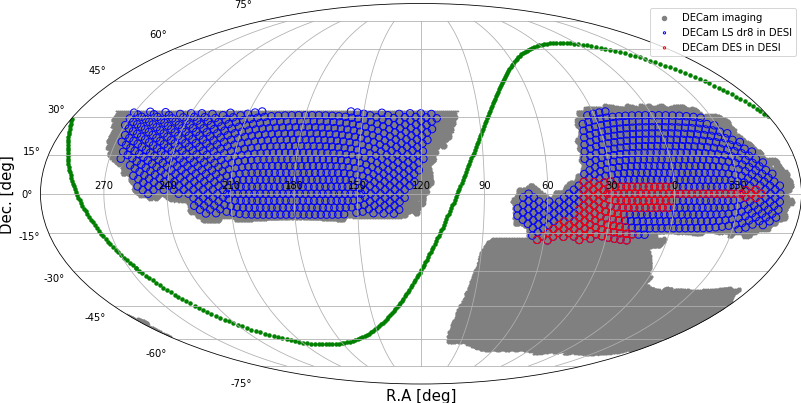
\includegraphics[width=\columnwidth]{images/decals_in_desi_footprint}
    \caption{Sky map of \DECam imaging footprint responsible of the \DECaLS data is shown in gray. The circles comprises the \DESI tiles and hence the \DESI footprint for \DECaLS data coming from LS \DECam  imaging in blue and from DES \DECam imaging in red.}
    \label{fig:decals_in_desi}

    \mike{I'll raise this as a broader point, but it's not clear to me that it wouldn't be better to look at the SV dataset to sample a wider range of conditions.}
\end{figure}


In order to fulfill the target classes required for the \DESI cosmology programme (\BGS, \LRGs, \ELGs and \QSOs), it was concluded that a three-band $grz$ optical imaging programme, complemented by \WISE \Wone and \Wtwo photometry, would be sufficient to select all target classes. The minimal  depth\footnote{The depths are defined as the optimal-extraction (forced-photometry) depths for a galaxy near the depth limits of \DESI, where that galaxy is defined to be an exponential profile with a half-light radius of $r_{\rm half}= 0.45$~arcsec.} required is $g=24.0$,$r=23.4$ and $z=22.5$. The minimum number of visits for this is 2. \DECam can reach these required depths in a total exposure times of $140$, $100$ and $200$ sec in g, r, z in nominal\footnote{Here ``nominal" is defined as photometric and clear skies with seeing FWHM of $1.3$~arcsec, airmass of $1.0$, and sky brightness of $22.04$, $20.91$ and $18.46$ AB mag arcsec$^{-2}$, respectively.} conditions.

\shaun{The imaging surveys have finished and so the numbers above should be what it did rather that what it aimed to do}


All data from the Legacy Surveys are first processed at \NOAO/Tucson\footnote{https://www.noao.edu/noao/staff/fvaldes/CPDocPrelim/PL201\_3.html} throughout the \NOAO Community Pipeline (\CP). Each instrument and telescope combination has its own \CP that takes raw data as an input and provides detrended and calibrated data products such as instrumental calibration (e.g., bias subtraction and flat fielding), astrometric calibration (e.g., mapping the distortions and providing a world coordinate system, or \WCS), photometric characterization (e.g., magnitude zero point calibration) and artifact identification, masking and/or removal (e.g., removal of cross-talk and pupil ghosts, and identification and masking of cosmic rays). 

The Legacy Surveys source catalogues are constructed using {\it Tractor}\footnote{https://github.com/dstndstn/tractor}(\cite{2016ascl.soft04008L}) throughout a post-processing catalogue generation pipeline called \LEGACYPIPE \footnote{https://github.com/legacysurvey/legacypipe}. \DESI Imaging Scientist Dustin Lang has developed the \TRACTOR forward-modelling approach to
perform source extraction on pixel-level data. This is a statistically rigorous approach to fitting the differing \PSF and pixel sampling of these data, which is particularly important as the optical data have a typical \PSF of $\approx 1$~arcsec.
The \TRACTOR takes as input the individual images from multiple exposures in multiple
bands, with different seeing in each. A simultaneous fit is performed for sources to the pixel-level data of all images. Thus, if a source is determined to be a point source, it is photometered as a point source in every band and every exposure. If it is found to be a morphologically extended source, then the same light profile is consistently fit in all images. This produces object fluxes and colours that are consistently-measured across the wide-area imaging surveys input to \DESI target selection. In general, The \TRACTOR improves target selection for all \DESI classes by allowing information from low signal-to-noise measurements to be utilized. The \TRACTOR catalogues will ultimately include source positions, fluxes, shape parameters, and morphological quantities that can be used to discriminate extended sources from point-sources, together with errors on these quantities. \BGS, being a flux-limited catalogue, will in principle require information of the flux only in the $r$-band. But, since we have tune the selection other \TRACTOR outputs have been brought in. The main \TRACTOR outputs required for \BGS comprises the fluxes\footnote{Fluxes outputs from \TRACTOR are in \NANOMAGIES. A flux of $1$ \NANOMAGIE corresponds to an AB magnitude of $22.5$.} in all the three bands ($g,r$ and $z$), the number of observations (\NOBS) in the three bands, the predicted flux (in the $r$-band only) within a fibre (\FIBERFLUX\footnote{\FIBERFLUX units are \NANOMAGIES}) in $1$~arcsec Gaussian seeing. The Galactic extinction values are derived from the \textsc{sfd98} maps \citep{1998ApJ...500..525S} and reported in linear units of transmission (\MWTRANSMISSION) in the $g,r$ and $z$ bands, with $1$ representing a fully transparent region of the Milky Way and $0$ representing a fully opaque region. The extinction coefficients for the \DECam filters were computed by Eddie Schlafly \citep{2011ApJ...737..103S} through airmass of $1.3$, computed for a $7000$K source spectrum. These coefficients are $A / E(B-V) = 3.995$, $3.214$, $2.165$, $1.592$, $1.211$, $1.064$ and then multiplied by the \textsc{sfd98} $E(B-V)$ values at the coordinates of each object to derive the $g, r$ and $z$ \MWTRANSMISSION values. And last the profile-weighted fraction information in the three bands; \FRACMASKED, \FRACFLUX and \FRACIN.

Fluxes in \TRACTOR transform to AB magnitudes as follows:
\begin{eqnarray}  
    mag^{*} \negthinspace &=& \negthinspace 22.5-2.5 \,\log_{10}(\FLUX) , \label{eq:mag_uncorr} \\
    mag^{\hphantom{*}}\negthinspace &=& \negthinspace 22.5 -2.5 \, \log_{10}(\CORRFLUX) , \label{eq:mag_corr}
\end{eqnarray}
where (\ref{eq:mag_uncorr}) does not correct for Galactic extinction while (\ref{eq:mag_corr}) does.

Regarding the completeness in the three bands of the \DECam Legacy Survey \DReight (\LS \DReight), in Table~\ref{tab:band_passes} it is shown the area covered for the different numbers of passes and in the different filters. These results involve data only within the \DESI footprint as of Figure~\ref{fig:decals_in_desi}. Our \DECaLS footprint covers a total of $9717$ deg$^2$, this translates to a $\sim 99.5 \%$ completeness in all the three bands (g,r,z) for at least one pass, $\sim 95.3 \%$ completeness for at least two passes and $\sim 70.7 \%$ completeness for at least three passes.

\begin{table}[h!]
\centering
\begin{tabular}{ |p{3cm}||p{1.4cm}|p{1.4cm}|p{1.4cm}|  }
 \hline
 {\bf Band/Number of Passes} & $\geq 1$ & $\geq 2$ & $\geq 3$\\
 \hline
 $g$-band   & $9687$ deg$^2$ & $9454$ deg$^2$ & $7769$ deg$^2$ \\
 $r$-band   & $9686$ deg$^2$ & $9422$ deg$^2$ & $7569$ deg$^2$ \\
 $z$-band   & $9686$ deg$^2$ & $9487$ deg$^2$ & $8036$ deg$^2$ \\
 All bands jointly & $9669$ deg$^2$ & $9257$ deg$^2$ & $6869$ deg$^2$ \\
 \hline
\end{tabular}
\caption{The table indicates the area covered by \DECam in Legacy Survey \DReight and in \DES survey for different numbers of passes and in different filters. We have restricted our results to data within the \DESI footprint as of Figure~\ref{fig:decals_in_desi}.}
\label{tab:band_passes}
\end{table}

\mike{I'll raise this as a broader point, but it's not clear to me that it wouldn't be better to look at the SV dataset to sample a wider range of conditions.}

\subsection{Tycho 2}

The mask that vetos objects near bright stars is partially-based on the \Tycho catalogue \citep{2000A&A...355L..27H}. The Tycho2 catalogue is an astronomical catalogue of more than $2.5$~million of the brightest stars. The catalogue contains positions, proper motions, and two-colour photometric data for $2,539,913$ of the brightest stars in the Milky Way, of which about $9000$ are visible to the naked eye.

\subsection{GAIA DR2}\label{subsec:gaia}

\GAIA \citep{2016A&A...595A...1G} is an \ESA space mission launched in 2013 with the aim of observe one billion stars ($\sim 1 \%$ of the total Milky Way stars) and to provide accurate positions, radial velocities, and optical spectrophotometry. The wavelength coverage of the astrometric instrument, defined by the white-light photometric $G$-band magnitude, is in the range $105$ - $330$~nm \citep{2016A&A...595A...7C}. These photometric data have a high signal-to-noise ratio and are particularly  suitable  for  variability  studies.

Since the first release of \GAIA in 2016 \citep{2016A&A...595A...2G}, the data
has been widely used by the \DESI Legacy Imaging Survey (i.e., for astrometric calibrations, proper motions, bright star masking) and is also ideal for constructing a star-galaxy separator for the \BGS. 
\GAIA covers the whole sky and is complete as faint as $G < 20.7$ which is sufficiently deep to detect all stars that might contaminate the \BGSF sample. We describe how we use a combination of \GAIA and \LS photometry to perform star-galaxy separation in Section~\ref{subsec:star_galaxy}.

\subsection{LSLGA}\label{subsec:LSLGA}

The Legacy Survey Large Galaxy Atlas (\LSLGA)\footnote{https://github.com/moustakas/LSLGA} is an ongoing project led by John Moustakas and Dustin Lang to select the largest galaxies in the \LS using optical data from the HyperLeda catalogue (\citet{2014A&A...570A..13M}) and infrared data from the \ALLWISE catalogue \citep{2015ApJS..221...12S}. Currently the catalogue contains $535,292$ galaxies that have a angular diameter (at the $25$~mag/arcsec$^2$ isophote) larger than $20$~arcsec.

\subsection{Globular Clusters}

Globular clusters in the \LS are identified using the Open\NGC catalogue\footnote{https://github.com/mattiaverga/OpenNGC} which contains NGC/IC objects. Open\NGC contains data from different databases: \NASA/\IPAC, HyperLeda, \textsc{simbad}, \textsc{heasarc}.

\shaun{We need to say a bit more about what globular Clusters are in this catalogue, i.e. give some stats. From the name it sounds like it is restricted to the NGC which wouldn't be good}

\section{Spatial Masking}\label{sec:spatial_masking}

Our main goal is to produce a reliable \BGS input catalogue for \DESI that fulfills the science requirements. To achieve this we must mask around bright stars where extended halos, ghosts, bleed trails and diffraction spikes around the stars can compromise the photometry of neighbouring objects. Similarly we must mask around very large galaxies  and globular clusters  that can also compromise the photometric measurements of their neighbours. 

Within the same framework, we have to propagate the instrumental effects such as saturated pixels, bad pixels, bleed trails, etc. that the \NOAO \CP tracks and \TRACTOR includes in the \LS catalogue\footnote{In \LS \DReight catalogue information on whether an object parameters have the possibility of being influenced by a bad pixel is flagged by the \ALLMASK \& \ANYMASK \MASKBITS.} 

One way to avoid contamination of the catalogue and possibility of wasting spectroscopic fibres on spurious targets around bright stars and galaxies
is by masking them around with simple but effective circular mask for stars and elliptical masks for galaxies. In \ref{subsec:geometric} we detail the geometrical masking functions we have applied on bright stars, in Large Galaxies and in Globular cluster to minimize the amount of spurious targets in our \BGS catalogue.  In \ref{subsec:pix_masking} we detailed the masks applied to reduce the number of spurious targets due bad pixels. 

It is very important to keep record of the fraction of the survey that is removed by these masks for extragalactic studies (i.e., clustering statistics) and for this we have made use of the RANDOM catalogue developed by the \DESITARGET\footnote{https://github.com/desihub/desitarget} team. The RANDOM catalogue has a density of $5000$ deg$^{-2}$ and include some of the information of the survey extracted from pixels at each random location, i.e., number of observations (\NOBSG, \NOBSR, \NOBSZ), galactic extinction (\EBV), the bitwise mask for optical data (\MASKBITS), etc\footnote{For more info on the randoms see: http://legacysurvey.org/dr8/files/\#random\-catalogs}.

\mike{Quote random density per pixel and per typical target?}
 
In figure \ref{fig:flow1} we show a flow chart summarizing the spatial masking applied for \BGS. The spatial masking was broken in two, the {\it Geometric Masking} and the {\it Pixel Masking}. The flow chart includes the area (in deg) and densities (in deg$^{-2}$) before and after applying the masks (blue boxes). The same information was recorded for the rejected objects (red boxes). The flow chart is sequential and must be read as the rows indicate this means the results of area and densities after the Pixel masking already include the Geometric masking. The same applies for the rejected objects in red boxes where objects rejected by the Pixel masking doesn't include objects rejected by the Geometric masking. In general, for our \DECaLS footprint of ~$9717$ deg$^2$, the spatial masking removes $\sim 3.07 \% $ of the area.

\begin{figure}
	%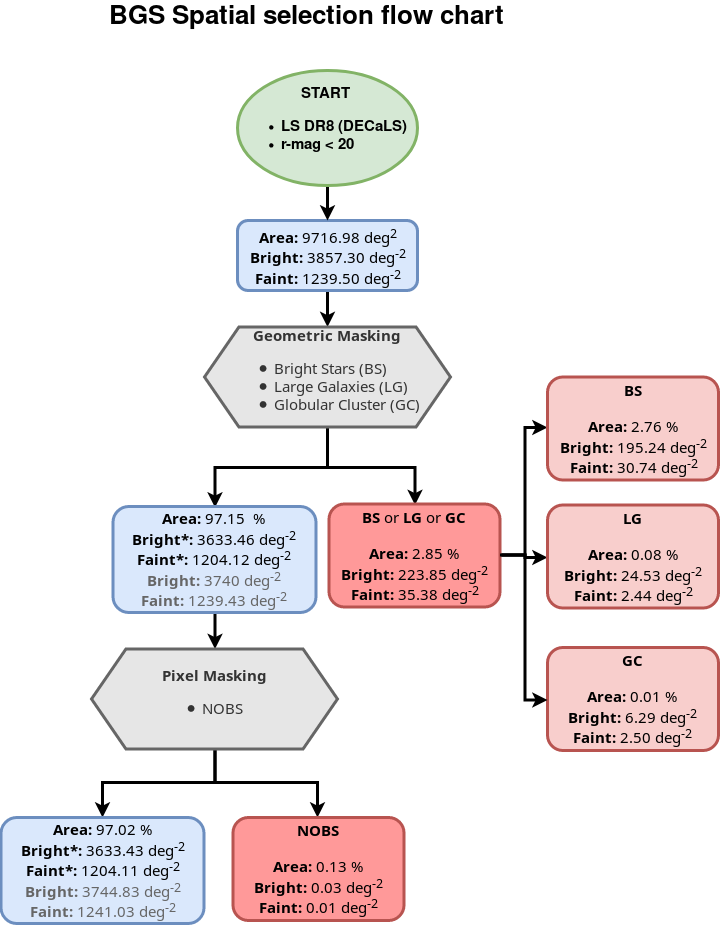
\includegraphics[width=\textwidth]{images/flow_geo}
	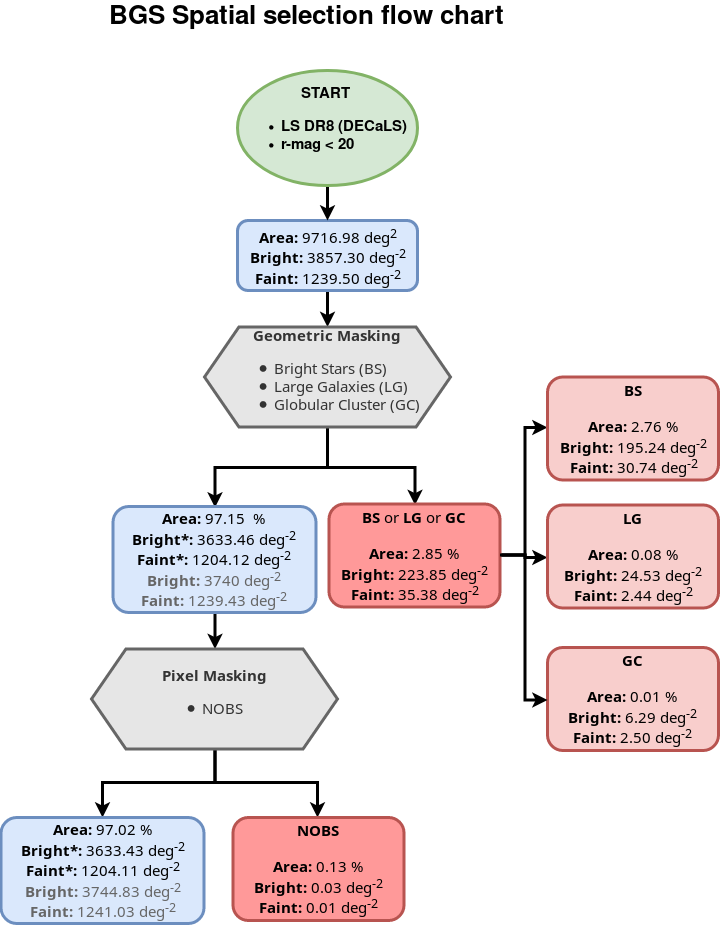
\includegraphics[width=\columnwidth]{images/flow_geo}
    \caption{Flow chart that shows the Spatial \BGS target selection in \DECaLS data from the Legacy Survey \DReight. The spatial selection of \BGS targets is divided in two kinds, one defined by the geometric-based cuts of the bright sources (Bright Stars, Large Galaxies and Globular Clusters), and by pixel-based cuts such as the number of observations (\NOBS). The flow chart shows the area (in deg) and number density (per square deg) broken into bright and faint before and after each of the \BGS cuts classes as blue, while in red it is shown the same information but for the removed objects. If more than one type of masking is presented at each stage (each of the gray hexagon boxes), then the dark-red boxes shows the results for the combination of the masks avoiding overlaps (as is the case of the Geometric Masking) and the light-red boxes shows the results for each individual mask. The upper ($^*$) in blue rectangles shows the target densities without the corrected area by previous masks while densities with not upper ($^*$) does account for previous masking for the area. Gray hexagon boxes show the different masking classes.}
    \label{fig:flow1}
\end{figure}

\subsection{Geometric}\label{subsec:geometric}
\subsubsection{Bright Stars}

The bright star mask is based on a combination of stars from \GAIA DR2 \citep{2018A&A...616A...1G} and Tycho 2 \citep{2000A&A...355L..27H} sources after correcting epoch and proper motions. This mask consists of predefined circular mask defined by the magnitude-radii relation,
\begin{equation}
\label{eq:mag_radii_bs}
  R_{\rm BS}(m) =
\begin{cases}
  39.3 \times 2.5^{(11 - m)/3} \, {\rm arcsec}, \hspace{0.6cm} m > 2.9 \\
   471.6 \, {\rm arcsec}, \hspace{3cm} m < 2.9
\end{cases}
\end{equation}
\mike{Is the 471~arcsec limit implemented in \DESI, or is this your implementation?  I didn't see it in \TRACTOR.}
\shaun{also double check the numbers as I expressed them in arcsec to make it more meaningful. They don't quite match at $m=2.9$}

\omar{Mike: its implemented but in degrees rather than arcsec here \url{https://github.com/legacysurvey/legacypipe/blob/master/py/legacypipe/reference.py\#L196}}

\omar{Shaun: I did it and it behaves the same as original. At $m=2.9$ radii is $466.47$ arcsec and at $m=2.89$ it is $467.9 arcsec$ a bit below than the $471.6$ arcsec.}

The \BS masking uses a total of $773673$ \GAIA DR2 objects ($\sim 82$ deg$^{-2}$) between with \GAIA $G$-mag down to $13$, while from \Tycho, we have a total of $3349$ objects ($\sim 0.36$ deg$^{-2}$) down to visual magnitude  \textsc{mag}\_\textsc{vt} of $13$. In order to avoid overlaps with \GAIA both catalogues have been matched applying proper motions to bring \GAIA objects to the same epoch of \Tycho and keeping the \Tycho objects that are not found in \GAIA. Then the magnitude, $m$ used in equation (\ref{eq:mag_radii_bs}) to mask around is a mixture of \Tycho visual magnitude, \textsc{mag}\_\textsc{vt}, and the \GAIA $G$-band magnitude. Within $R_{\rm BS}$ \TRACTOR forces all the sources it detects to be fit the \PSF profile to avoid artificially fitting diffraction spikes and stellar haloes as large extended sources. Thus any galaxies detected within $R_{\rm BS}$ will have their 
fluxes underestimated. Consequently to define a clean galaxy catalogue we must veto all sources within  $R_{\rm BS}$ of a bright star. In Fig~(\ref{fig:flow1}) we show that this Bright star mask covers $2.85$ \% of the initial footprint and rejects $\sim 224$ bright objects/deg$^{2}$ and $\sim 35$ faint objects/deg$^{2}$ when averaged over that full initial footprint.

\shaun{There are several things I'm confused about in the following.  Is it the stars themselves that have \BRIGHT set or the objects within $R_{\rm BS}$? What is set for the \Tycho stars. Is the PSF only fitting done for objects with $R_{\rm BS}$ of \GAIA star even when it is not a \Tycho star. }
\mike{The \GAIA stars have the \BRIGHT bit set only if they do not already match with a \Tycho  source. Don't understand what this means}
\mike{Probably should mention the epoch matching.}
\omar{I have edited above text and hopefully it is more clear now.}
\omar{I have a concern regarding the area computed throughout the flow charts, $$A = A \cdot N_{ran}^{mask}/N_{ran} = N_{ran}^{mask} \cdot \eta_{ran}^{-1}$$ where $\eta_{ran}=15000$ is the number density of the randoms and $N_{ran}^{mask}$ is the number of objects kept or rejected by a particular mask (i.e., \BS, \LG, \NOBS). This way is different from the way we get the area with pixels, $$A = A_{pix}\cdot\sum f_{A}$$, where $f_{A} \equiv A_{pix}^{-1}\cdot N_{pix}/\eta_{ran}$ is the fractional area, $N_{pix}$ is the number of objects within the pixel after applying the masks, $\eta_{ran}=15000$ is the density of the randoms without any mask ($5000$ deg$^{-2}$ per file) and $A_{pix}^{-1}$ is the area of the pixel $0.052$ deg$^2$ in this case. Using the flow chart way, we end up with a total reduced area of $9428.38$ deg$^{2}$ while with the pixel way $9401.05$ deg$^{2}$.}

%%%%%%%%%%%%%%
\begin{figure*}
	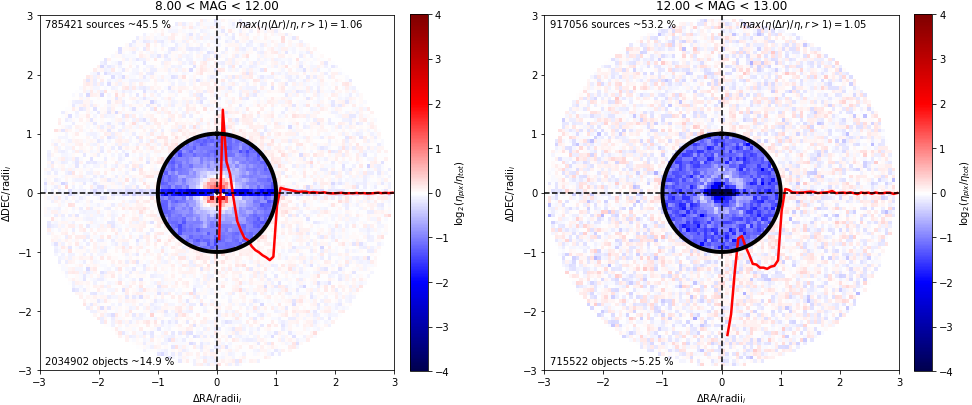
\includegraphics[width=16cm]{images/2dstack_reescaled_bs_south_nobsmask}
	%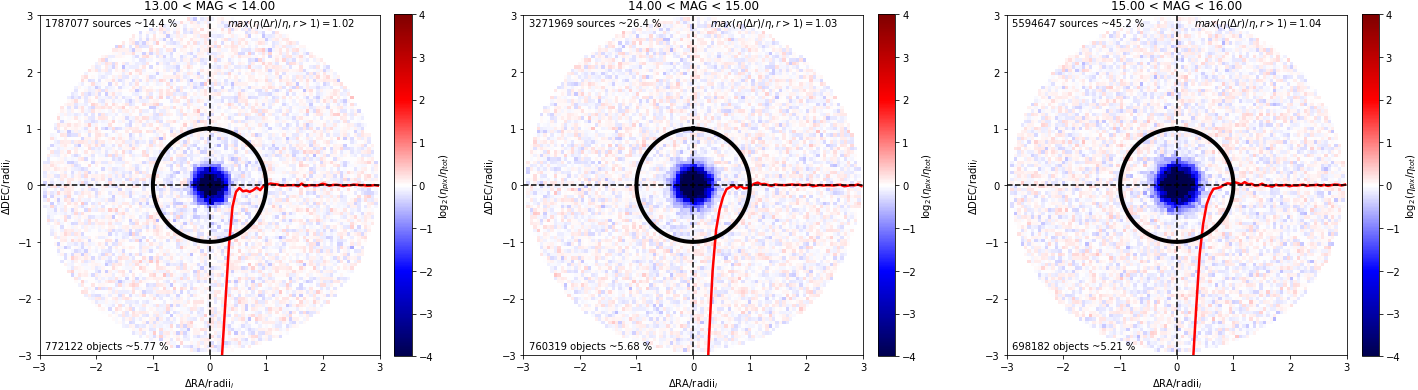
\includegraphics[width=16cm]{images/2dstack_reescaled_ms_south_withbsmask.png}
    \caption{2D stacks of \BGS objects around \BS sources composed of \GAIA and \Tycho sources down to $G$-mag and visual magnitude \textsc{mag}\_\textsc{vt} of $13$ respectively. From the \BGS side, we have not set the \BS bit to account for the amount of contamination. The stacking was broken into magnitudes in the \BS sources catalogue from $8$ to $12$ (left) and $12$ to $13$ (right). The stacking was rescaled to the masking radius function of equation \ref{eq:mag_radii_bs}, meaning that objects within $0$ and $1$ will be mask out by the \BS bit while objects with $r/R_{\rm BS} > 1$ will survive the \BS bit (here $r^2 = \Delta RA^2 + \Delta DEC^2$). The colour distribution shows the density ratio of the density per pixel ($\eta_{pix}$) and the total density ($\eta_{tot}$) within the shell $1.1 < r/R_{\rm BS} < 3$. The density ratio is shown on a $\log_2$ scale where red shows the over-densities, blue the under-densities and white the mean density. The black solid circle shows the \BS bit threshold and the red solid line is the over-densities radial profile with same scale as the as the colour distribution $\log_2(\eta_i/\eta_{tot})$ where $\eta_i = \sum \eta_{pix}(\Delta R)/N_{pix}(\Delta R)$, $N_{pix}(\Delta R)$ is the number of pixels within the annulus $\Delta R$ and $R$ being the stacking scaled axis $r/R_{\rm BS}$. Bottom panel: 2D stacks of final \BGS sample (with \BS bit set on) and the so called \MS bit which contains the \BS bit and fainter \GAIA sources down to $G$-mag $16$. Here we show the stacking for magnitudes in the \MS bit source catalogue from $13$ to $14$ (left), $14$ to $15$ (middle) and $15$ to $16$ (right).}
    \label{fig:2dstack_tycho_reescaled}
\end{figure*}

To determine whether this bright star mask is adequate or whether the effects of stellar haloes on the photometry of neighbouring galaxies extends to larger radii,  in Fig.~\ref{fig:2dstack_tycho_reescaled}  we have made stacks of the BGS galaxies around the bright stars prior to applying the bright star mask.
The stacks were made by expressing the angular separation of the \BGS galaxies from the their nearest bright star in units of the
bright star masking radius $R_{\rm BS}$.
In these rescaled coordinates, galaxies within a radius of $1$, shown by the black circle, are in the BS masking zone.
We show stacks for two MAG\_VT bins, one with bright stars of magnitude between $8$ to $10$ and one fainter with magnitude between $10$ to $12$. The radial profile (red solid line) shows the variation in the target density, defined as $\Delta\rho(R) \equiv {\eta}(r)/\bar\eta - 1$ where ${\eta}(r)$ is target density in an annulus at radius $R$ and $\bar\eta$ is the mean target density
evaluated over the region $1.1 < R < 3$. This means $\Delta\rho(R) = 0$ corresponds to a mean density, $\rho(\Delta R) \ge 1$ to overdensities at least twice the mean density, and $\Delta\rho(R) < 0$ to underdensities. The large underdensity at radius $R \le 1$ is due to \TRACTOR forcing all objects within this region to be fit as \PSFs. Note that before applying the mask we would still have some \BGS targets with $R_{\rm BS}$ as star-galaxy separation for \BGS is not determined by the \TRACTOR \PSF designation.
In each panel of the panels of 
Fig.~\ref{fig:2dstack_tycho_reescaled}, we see a spike up spurious sources for $R < 0.2$.
\shaun{Need to describe what we see at $R>1$ in the updated versions of these plots}


\subsubsection{Large Galaxies}

As opposed to the circular masking around BS, the masking around Large Galaxies (LG) consists of predefined elliptical masks taken from the LSLGA catalogue (see \ref{subsec:LSLGA}).

The LG mask is way less aggressive than the BS mask, rejecting only $0.13 \%$ of initial area which $~33$ deg$^{-2}$ of those are bright objects and $~3$ deg$^{-2}$ are faint.

\omar{include more info here...}

\subsubsection{Globular Clusters}

The globular cluster (GC) mask works similar to the BS mask and apply predefined circular mask. The masking radius is defined by the majax attribute of the OpenNGC catalogue.

The GC mask has the smallest impact of the geometric masks, rejecting only $0.02 \%$ of initial area along with  $~15$ bright galaxies deg$^{-2}$ and $~5$ faint galaxies deg$^{-2}$.

\omar{more info here too...}

\subsection{Pixel}\label{subsec:pix_masking}
Some of the effects that compromises the pixels and the model fitting itself includes bad pixels, saturation, cosmic rays, bleed trails, transients, etc. The NOAO DECam CP identifies these instrumental effects during their various calibrations\footnote{The document that lists all the calibrations and has details on the various maska can be found at: \url{https://www.noao.edu/noao/staff/fvaldes/CPDocPrelim/PL201\_3.html}} (see Table $5$ in \cite{2019AJ....157..168D} for the various calibratioons) and these are passed through \TRACTOR and compiled in the \ALLMASK bitmask\footnote{Details of this bitmask can be found here: http://legacysurvey.org/\DReight/bitmasks/\#id3}. \ALLMASK denotes a source that touches a bad pixel in all of a set of overlapping images.
%ANYMASK denotes a source that touches a bad pixel (a pixel that presents any of these effects) in any of a set of overlapping images
\mike{Do we use/need to discuss ANY?}
\omar{You're right, we don't use ANY. I've remove it.}

Besides the bad pixels due instrumental defects, \BGS require a complete sample in the three bands ($g, r, z$) and therefore we impose at least one observation in each of the bands the \NOBS parameter. Both, \ALLMASK and \NOBS are pixel-based and hence these information is also available in the RANDOMS. However, we find out that virtually all the area ($~97\%$) (and hence randoms) rejected by \ALLMASK is also rejected by the \NOBS$=0$ (in any band). In addition \ALLMASK rejects significant number of objects ($196$ deg$^{-2}$) but with very little associated area ($~0.01\%$ of the full area). Virtually all the objects \ALLMASK rejects and many more are rejected by the quality cuts in \FRACMASKED, \FRACIN and \FRACFLUX (in any band) that we are already applying and we will review in section \ref{sec:photo_select}. 

In conclusion, there is little to be gained from using \ALLMASK and we decided to use only \NOBS as our pixel-base mask shrinking the area by $0.13 \%$ and reducing the target density by a $0.03$ deg$^{-2}$ for bright objects and $0.01$ deg$^{-2}$ for faint objects.

\section{Photometric Selection}\label{sec:photo_select}

The second class of \BGS targets comprehend the selection based on its photometry. According to the science requirements for \BGS and mocks \citep{Smith:2017tzz}, it is expected to have a target density of $~800$ deg$^{2}$ for a $r$-band limit of 19.5. For the faint sample (19.5 > $r$-band > 20) and second priority in \BGS as part of the Bright Time Survey (BTS), it is expected a density of $~600$ deg$^{2}$.

\begin{figure}
	%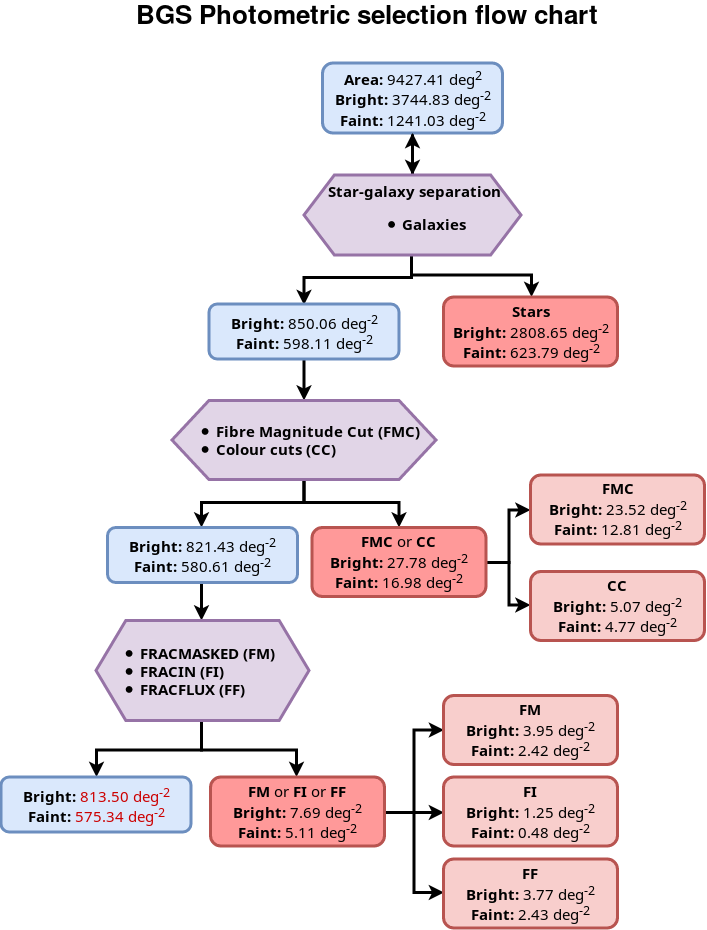
\includegraphics[scale=0.4]{images/flow_phot}
	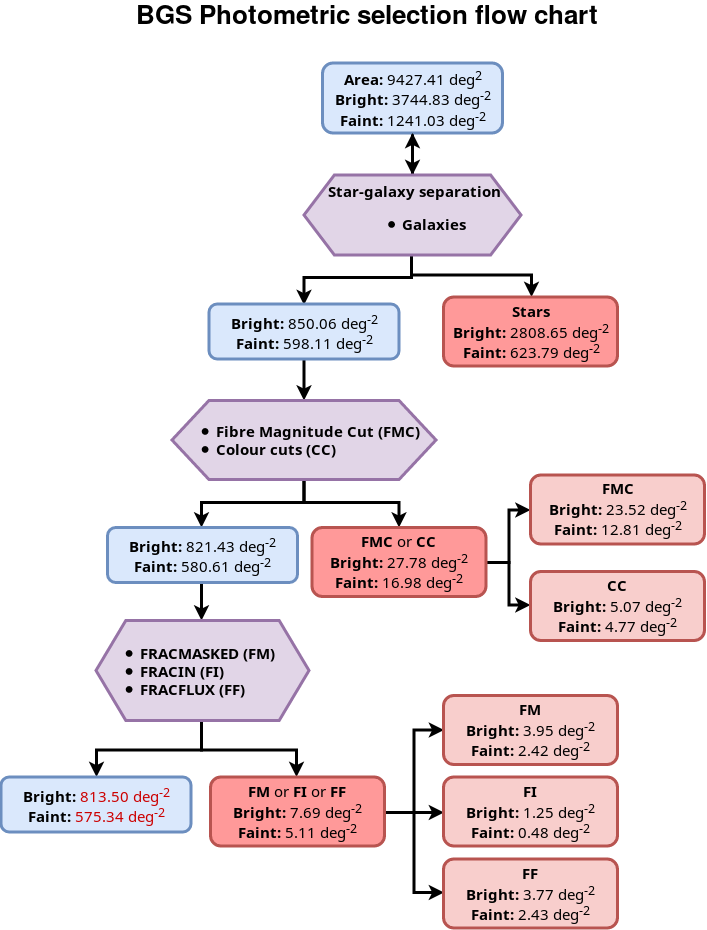
\includegraphics[width=\columnwidth]{images/flow_phot.png}
    \caption{Flow chart of \BGS target selection in the Legacy Survey \DReight based on photometric selections. The photometric selection of \BGS targets is divided in four kinds; Star-Galaxy separation, Fibre Magnitude Cuts (\FMC), Colour Cuts (\CC) and Quality Cuts (\QCs). The photometric-based flow chart is a continuation of the spatial-based flow chart (see figure \ref{fig:flow1}) and therefore we start with the area and densities where we left in the spatial-based flow chart. We break densities into bright and faint and shows the outputs after each of the \BGS cuts classes as blue. In red it is shown the densities of the removed objects and in yellow it is shown the different cut classes.}
    \label{fig:flow2}
\end{figure}

One of the major challenges for \BGS is the separation of stars and galaxies. In this work we took advantage of \GAIA DR2 \citep{2018A&A...616A...1G} along with \TRACTOR best-fit model to classify stars and galaxies. 

\DESI \BGS has minimal risks regarding redshift success rates compared to other targets in \DESI.  
\mike{This may prove to be optimistic!}

\TRACTOR incorporate a simulated fibre flux in the three bands ($g,r$ and $z$) computed using the model data at $1$ arcsec Gaussian seeing. We use this parameter in the $r$-band to bail out spurious galaxies motivated by eye inspections. 
 
%However, a possible risk according to survey simulations suggest a lack of star forming objects at a fixed observing condition (add cite...). Another possible source of incompleteness is low surface brightness objects, which become more difficult to observe under bright time conditions (add cite...). We try to minimize this problem by imposing a cut in FIBERFLUX in the $r$-band.

Posterior photometric-based cuts includes colour outliers in $g-r$ and $r-z$ and some quality cuts that relies on the low accuracy in its flux measurement. Such quality cuts are based on \FRACMASKED, \FRACFLUX and \FRACIN \TRACTOR outputs in any of the three bands.

\begin{figure*}
	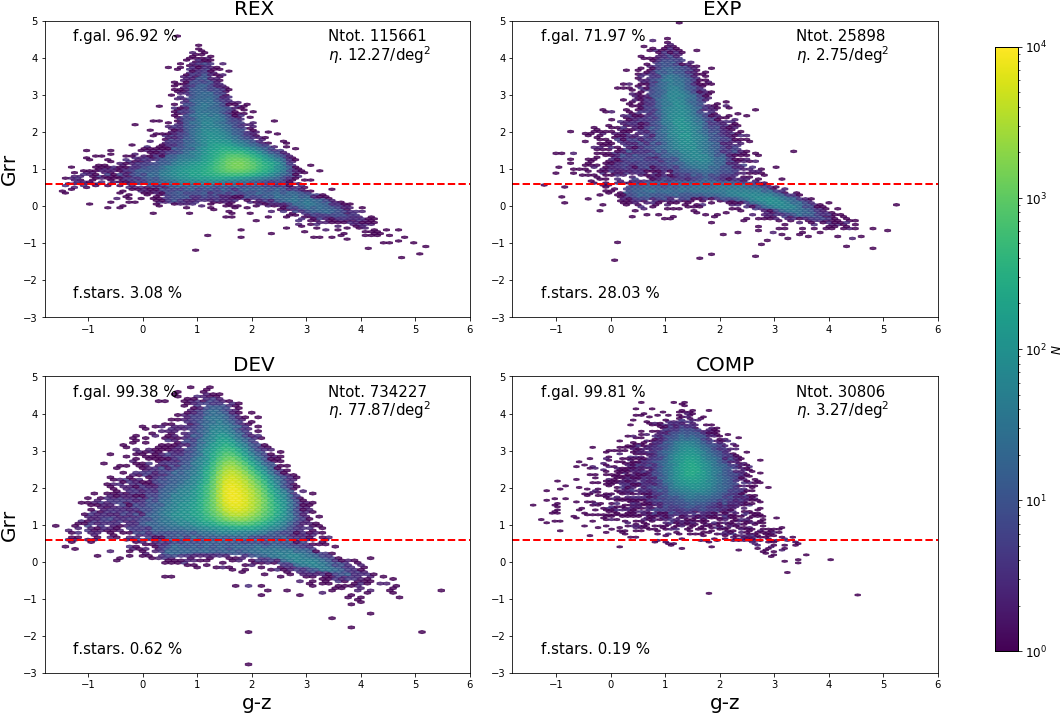
\includegraphics[width=12cm]{images/gz_Grr_bgsbutsg_hexbin_extended}
	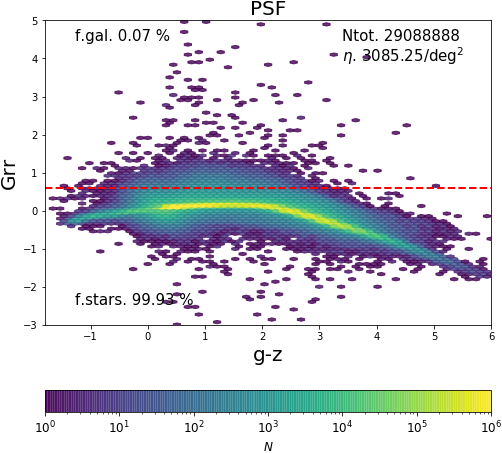
\includegraphics[width=5cm]{images/gz_Grr_bgsbutsg_hexbin_psf}
	%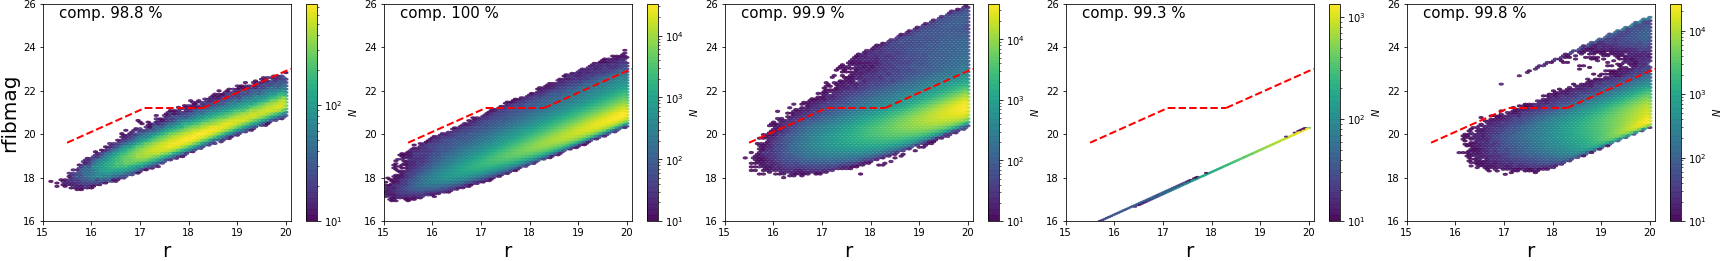
\includegraphics[width=17cm]{images/r_rfibmag_bgsbutfmc_hexbin}
	%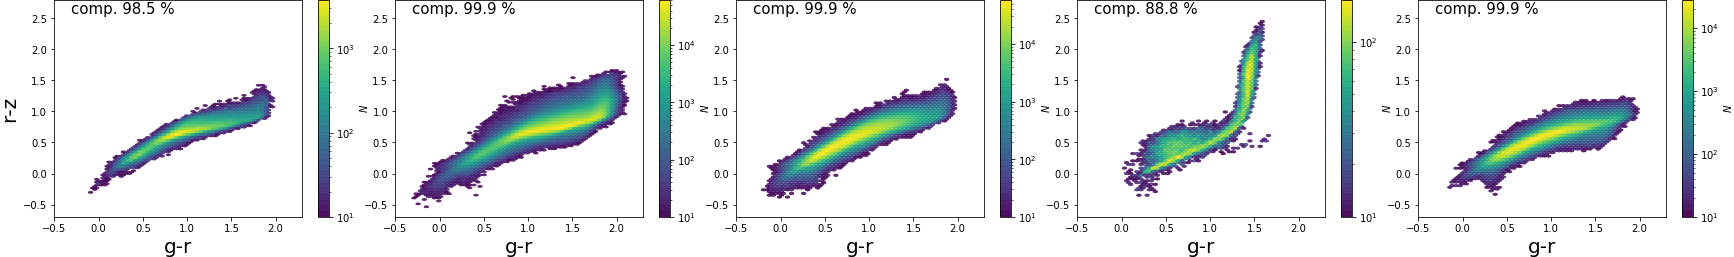
\includegraphics[width=17cm]{images/gr_rz_bgs_hexbin}
    \caption{Colour-colour plot $g-z$ and $G-rr$ of stars and galaxies according to the \GAIA classification after the Geometric and Pixel cuts of the spatial-based cuts (see  figure \ref{fig:flow1}) and after the photometric-based cuts (see figure \ref{fig:flow2}) except from the Star-galaxy separation cut itself. $G$ is the \GAIA $G$-band photometric magnitude from the \GAIA DR2 catalogue and $rr$ is the $r$-band magnitude from the LS \DReight without extinction correction. $g$ and $z$ are the $g$-band and $z$-band magnitudes from the LS \DReight catalogues with extinction corrections both. The plots shows cross-matched LS \DReight objects with \GAIA DR2 only and was broken in the five morphology classes from \TRACTOR best-fitting model. The red-dashed line draws the threshold limit at $G-rr = 0.6$ for stars and galaxies ($G-rr < 0.6$ for stars and $G-rr > 0.6$ for galaxies). The colour in the plots show the number counts ranging from $1$ to $5000$ objects except for thr PSF-type objects which goes from $1$ to $2$ Millions. We have included the fraction of galaxies and stars according to this classification at the top-left corner and bottom-left corner respectively. The total amount of objects within each plot and the target density is at top-right corner.}

    \mike{Don't you need to distinguish the objects enforced to be \TRACTOR PSF by the \GAIA AEN criteria?  Otherwise, it's a bit misleading.}
    \mike{It's not obvious to me why it's more correct to not account for extinction in $Grr$?}
    \mike{I think it's the case that:  you believe a colour cut is better than AEN and that you'd rather use colours than depend on \TRACTOR PSF (due to the seeing dependence?) but I don't see an argument along these lines being made in the text?}
    
\omar{I've modified the text and hope it's clearer now.}
    \label{fig:Grr-gz}
\end{figure*}

In figure \ref{fig:flow2}  we show the second part of the \BGS target selection flow chart. This flow chart focuses on the photometric selections and start where we left in previous spatial selection. Our \BGS catalogue end up having a reduced area of $1348.04$ deg$^{2}$ and target densities of $846.88$ deg$^{-2}$ and $592.62$ deg$^{-2}$ for bright and faint objects respectively. 

\subsection{Star-Galaxy Separation}\label{subsec:star_galaxy}

Many efforts have been made in star-galaxy classification since the beginning of the multi-object spectroscopy era, these include algorithms using machine learning methods i.e., Neural Network algorithm (cite NN examples), Support Vector Machine (SVM) (cite SVM examples) and Random Forests (cite RF examples), algorithms using pixel-level flux measurements i.e., Normalised Linear Discriminant (cite example), and template fitting i.e., Template fitting of spectral energy distribution (cite example). However, rather than look at the morphology given by \TRACTOR to select stars and galaxies we divided our classification using \GAIA DR2 detections. 

\GAIA \citep{2016A&A...595A...1G}, as mentioned in section \ref{subsec:gaia}, is a space-base survey aim to make a three-dimensional map of our Galaxy, the Milky Way. \GAIA has observed $~1.7$ billion stars in the second data release (DR2)\footnote{DR2 cover 22 months of observations and was release on 25 April 2018.} with a limiting magnitude of $20.7$ in the $G_{\rm{GAIA}}$-band. \GAIA, as a space-base survey does not have to deal with ground-based systematics like seeing, which affects considerably the measurements in the PSF, fluxes and morphology. \GAIA data processing includes self-calibrating that allows calibration in the PSF model \citep{2016A&A...595A...1G}. Systematic astrometric errors (averaged over the sky) in \GAIA are at the level of $<0.1$ mas while astrometric residuals in the LS \DReight are of the order of $\pm 0.03$ arcsec. \GAIA DR2 is widely used in the LS \DReight for astrometry calibrations and masking. \GAIA has been made available in the LS catalogues since the LS DR7.

\omar{do we need to include information regarding the matching between \GAIA and \TRACTOR i.e., the matching distance, epoch corrections, etc.?}

\begin{figure*}
	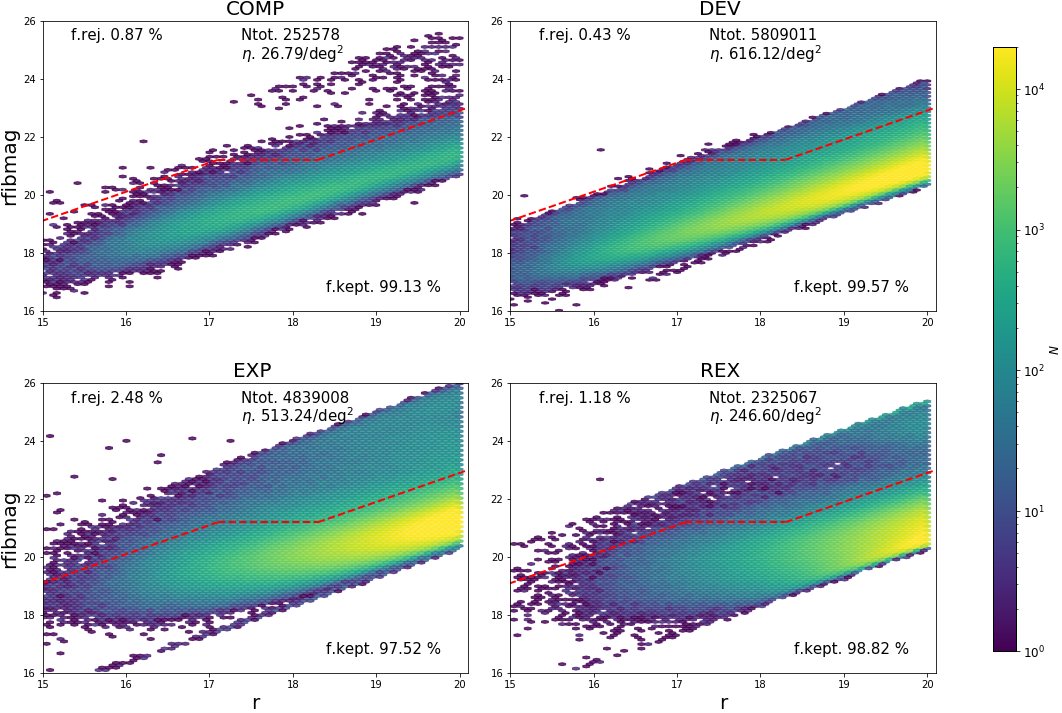
\includegraphics[width=12cm]{images/r_rfibmag_bgsbutfmc_hexbin_extended}
	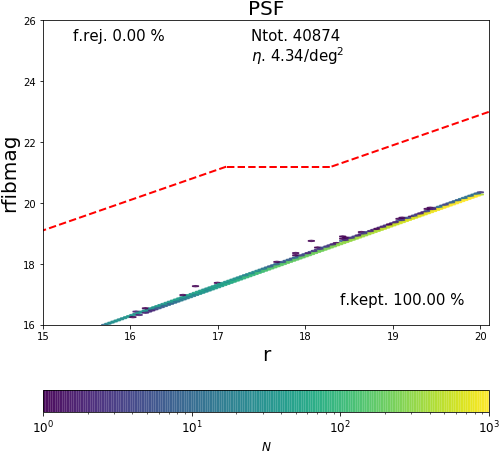
\includegraphics[width=5cm]{images/r_rfibmag_bgsbutfmc_hexbin_psf}
    \caption{ \BGS galaxies in the $r$-band total magnitude versus $r$-band fibre magnitude from the LS \DReight. The results were divided into the five different \TRACTOR best-fit morphology model. The colour bar shows the number counts ranging from $1$ to $20,000$ for four of the best-fit models with the exception of the PSF-type galaxies that runs from $1$ to $2000$. The red-dashed line shows the \FMC cut where we reject everything that is above that threshold. Number on top-left and bottom-right corner are the fraction of galaxies rejected and kept respectively while numbers at top-right corner shows the total number of galaxies and its target density.}
    \label{fig:fmc}
\end{figure*}

\GAIA main task is to select stars but yet some galaxies pass throughout the selection algorithm (cite https://www.aanda.org/articles/aa/pdf/2014/08/aa23514-14.pdf) although the number of galaxies spotted by \GAIA remains small. \omar{check fraction of galaxies in \GAIA from above paper if any.} Using \GAIA DR2 as truth table for stars, we based or galaxy classification in two parts,

\begin{itemize}
    \item $G-rr > 0.6$.
    \item Objects not in \GAIA.
\end{itemize}

The $G$-band is the G photometric \GAIA magnitude and $rr$ is the $r$-band magnitude from the LS \DReight without extinction correction. The election of taking the difference $G-rr$ is driven by the fact that $G$-band in \GAIA is centred at the relatively same position as the $r$-band in the \LS with the only difference than the $G$-band is much broader than the $r$-band. We decided not to account for extinction correction in the $r$-band because we do not need to worry about dust for such close objects. Thus $G-rr$ separate the redder objects in \GAIA above zero. In figure \ref{fig:Grr-gz} we show a $g-z$ versus $G-rr$ colour plot of \GAIA only objects matched in LS \DReight and broken into the five morphology types \TRACTOR uses in their model fit. The cross-matched objects include all the \BGS cuts (i.e., Spatial and Photometric) with the eception of the Star-galaxy separation itself. From PSF-type objects, we can see the stellar locus around $G-rr=0$, while for the remain morphology types (COMP, DEV, EXP, REX) we see part of the galaxy locus\footnote{We have to remember that Fig.~\ref{fig:Grr-gz} only includes cross-matched stars and galaxies between \LS \DReight and \GAIA.} in the upper part of the plot, just above $G-rr=0$. 

It is clear from Fig.~\ref{fig:Grr-gz} that \TRACTOR morphology support the \GAIA classification but still we can see some remnants of the stellar locus for the non-PSF model-fitted objects. The agreement accounts for $99.93 \%$ for PSF-type objects and less than $3.1 \%$ disagreement for non-PSF type morphologies with the exception of the exponential (EXP) model-fit with the highest disagreement of $\sim 30 \%$. Using the \TRACTOR morphology and \GAIA $G$-band information we define our star-galaxy separation at the threshold limit of $0.6$ in $G-rr$. 

For future references we will refer to stars and galaxies to objects in the \LS \DReight that meet our \GAIA classification. 

The fraction of galaxies that are in \GAIA (objects above $0.6$ in $G-rr$ of figure ~\ref{fig:Grr-gz}) is $xx \%$ which is quite low compared to the total amount of galaxies.
\omar{Compute the fraction of galaxies cross-matched with gaia out of the total of galaxies}

\BGS target selection is taking the expected density after star-galaxy separation. From Spatial flow chart in figure \ref{fig:flow2}, we end up having a bright target density of $850.06$ deg$^{-2}$ and a faint target density of $598.11$ deg$^{-2}$. Meanwhile, rejected \GAIA stars have a target density of $2808.65$ deg$^{-2}$ bright stars and $623.79$ deg$^{-2}$ faint stars.

In Appendix~\ref{app:sgmodels} we compare the \GAIA star-galaxy classification with stars being selected by \TRACTOR PSF model type and with \TRACTOR current star-galaxy separation for \GAIA cross-matches using the \GAIA Astrometric Excess Noise.

\subsection{Fibre Magnitude Cut}
\mike{Is this implemented in DESI target?}
\omar{Yes. \url{https://github.com/desihub/desitarget/blob/master/py/desitarget/cuts.py\#L1090-L1092}}

In order to reduce the number of spurious galaxies caused by fragmented, shredded and imaging issues we apply a fibre limited cut defined as follows:

%low signal to noise and hence low redshift success rate target density, a surface brightness (SB) limit has been applied to the \BGS selection. The SB limit is given by the predicted Fibre Flux (refer to \TRACTOR paper, or any docummentation, where this FIBRE flux is defined...) and the total flux both in the $r$-band. The SB cut was defined as follows:

\begin{eqnarray}\label{eq:fmc}
    & [rfibmag < (2.9 + 1.2) + r  \hspace{3 mm} \text{AND} \hspace{1 mm} & rmag < 17.1 ] \nonumber \\
    & \text{OR} \hspace{3 mm} [rfibmag < 21.2 \hspace{3 mm} \text{AND} \hspace{1 mm} &17.1 < r < 18.3] \nonumber \\ 
    & \text{OR} \hspace{3 mm}  [rfibmag < 2.9 + r \hspace{3 mm} \text{AND} \hspace{1 mm} &r > 18.3]
\end{eqnarray}

where $rfibmag$ is the magnitude of the $r$-band fibre flux and $r$ is the total $r$-band magnitude both accounts for extinction correction. Equation~(\ref{eq:fmc}) defines the {\it fibre magnitude cut} (\FMC) and in figure~\ref{fig:fmc} we show this cut in the red-dashed line for \BGS galaxies in the $r$-band total magnitude versus $r$-band fibre magnitude plot broken into the five different \TRACTOR best-fit models. We kept everything below the red-dashed line affecting mostly galaxies with exponential (EXP) and round exponential (REX) best-fittings. 
\omar{Explain why do we have such a star-like objects behaviour in PSF galaxies as shown in Fig.~\ref{fig:fmc}. What are those objects? Do they represent the forced PSF fit objects?}

The \FMC was motivated by the huge amount of spurious galaxies found at high $rfibmag - r$ values that can be explained by a low surface brightness galaxies and a poor model fit. The threshold limit in equation~\ref{eq:fmc} was build based on eye inspection where we see at least $50 \%$ of good galaxies.

%Colours show whether a galaxy is PSF fitted (red-dots) or not (blue-dots). The \FMC was establish due eye inspection above the line $rfibmag > 2.9 + r$, below this line it is likely we have a high completeness in redshift success rate. At the bright end, for $r < 18.3$ it was found at least a $50 \%$ good objects and $~30 \%$ of Large Galaxies (from the LSLGA catalogue) above the $rfibmag > 2.9 + r$ line.  

This \FMC rejects an extra $36.33$ deg$^{-2}$ from previous cut (star-galaxy separation) of which $23.52$ deg$^{-2}$ are bright galaxies and $12.81$ deg$^{-2}$ are faint galaxies.

\subsection{Colour Cuts}

We also get rid of weird colours in galaxies. This are objects that falls far outside the galaxy locus in the $g-r$ versus $r-z$ colour-colour regime. The limits we have defined for the outliers are:

\begin{eqnarray}
    (-1 < g-r < 4) \nonumber \\
    \text{AND} \hspace{3mm} (-1 < r-z < 4).
\end{eqnarray}

The colour cut (\CC) rejects an additional $9.84$ deg$^{-2}$ of which $5.07$ deg$^{-2}$ are bright galaxies and $4.77$ deg$^{-2}$ are faint.

\subsection{Quality Cuts}

In section \ref{subsec:pix_masking} we mentioned that bad pixels, associated to bitmask cut, happened to be a subset of our Quality Cuts (\QCs). The \QCs are conformed by,

\begin{eqnarray}
    &\textsc{fracmask\_i}& < 0.4, \nonumber \\
    \text{AND} \hspace{3mm} &\textsc{fracin\_i}& > 0.3, \nonumber \\
    \text{AND} \hspace{3mm} &\textsc{fracflux\_i}& < 5, \hspace{1cm} i \equiv  \textrm{G, R and Z}
\end{eqnarray}

\FRACMASKED $< 0.4$ can be understood as objects with model not dominated by masked pixels where $0.4$ is the fraction of pixels masked and higher numbers indicate higher contamination. \FRACIN $> 0.3$ means that most of the model flux lies inside the region of the data used to fit the model. \FRACFLUX $< 5$ select objects not overwhelmed by neighbouring sources, this is, the flux from surrounded objects do not exceed five times the flux of the object itself.

Despite the \QCs information can not be passed through the RANDOMS, we find this cut extremely important as it complements most of the previous cuts. \FRACMASKED catch galaxies with low surface brightness that the \FMC missed and also objects near bright sources and spurious due fragmented bright objects. \FRACIN also spot low surface brightness galaxies as well as \FRACFLUX but \FRACFLUX also spot small regions of incompleteness in the three bands that could be due CCD gaps. We have decided to implement the \QCs at last so we can have a summary of how well the previous cuts works. Turns out they works great as \QCs rejects an additional of $12.8$ deg$^{2}$ of which $\sim 50 \%$ is due \FRACMASKED, $\sim 40 \%$ is due \FRACFLUX and the rest $(\sim 10 \%)$ correspond to \FRACIN.

\mike{I hope to come back to this, but it'd be nice to tidy up the fundamental origins of some of these.  E.g. there seems to be a large overlap with medium star masks?}
\omar{I haven't compare the overlap with medium star mask. We have decided that there's no need to apply the medium star masking but I think is worth to check if there's any overlap with the \QCs first.}

In  Appendix~\ref{app:galview} we change the order in which we implement the \BGS cuts putting at first place the star-galaxy separation which leave us with a galaxy view of the \BGS target selection. In addition to this change from the selection criteria order presented in this section, we swap the \FMC with the \QCs leading to a different view shown at flow chart in Fig.~\ref{fig:flow_galaxy}. 

%\subsection{Photometric Systematics}

\begin{figure*}
	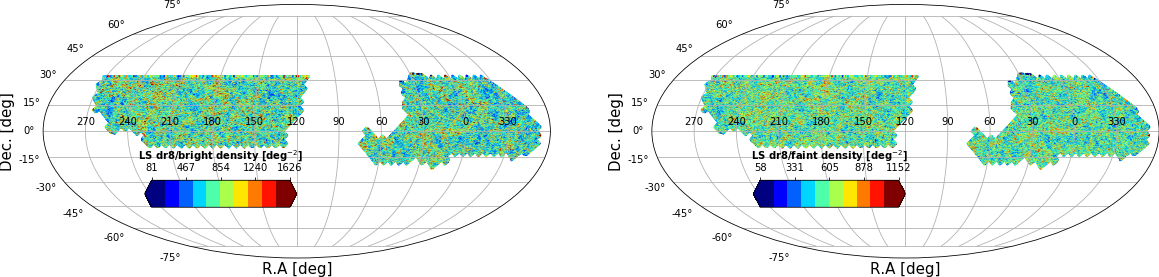
\includegraphics[width=17cm]{images/skymaps_bright_faint.png}
    \caption{Sky map...}
    \label{fig:skymap_densities}
\end{figure*}


\section{Catalogue Properties}
%\subsection{North Vs South}
As an initial assess of the \BGS target selection, we carried comparisons with the \GAMA Main Survey \citep{10.1093/mnras/stx3042} and with the MXXL light-cone catalogue \citep{Smith:2017tzz}. We compare the magnitude, target density and clustering properties. Using \GAMA redshifts, we asses our asses our star-galaxy classification and plot the cross-match redshift distribution. 

\subsection{Magnitude definition and redshift distribution with GAMA}

We use the \GAMA DR3 Main Survey, which has a $98.85 \%$ redshift completeness, to match with our \BGS target catalogue. In terms of the footprint and quality of the \GAMA data, we choose three out of the four \GAMA fields: G09, G12, G15, ignoring G02 as this is only partially covered by \DECaLS footprint. \GAMA main survey is complete to r petrosian (\RPETRO) of $19.8$ and to get reliable redshifts, we select targets with \GAMA \NQ with a value of $3$ or more. The area of each \GAMA field is $59.98$ deg$^2$ meaning that our matched sample has a total area of $\sim 180$ deg$^2$.

\begin{figure*}
	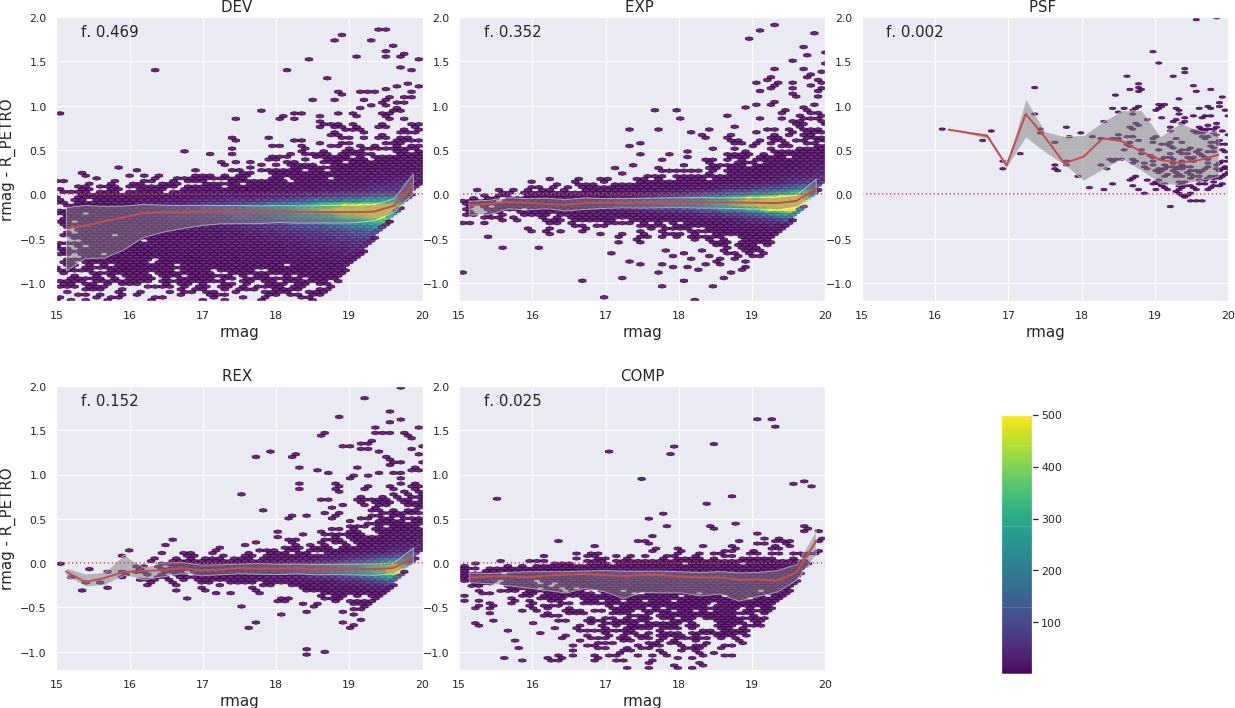
\includegraphics[width=17cm]{images/bgs_gama_mag_diff}
    \caption{ $r$ vs $r-\RPETRO$ for \BGS galaxies cross-matched with \GAMA. $r$ is the $r$-band magnitude from the LS \DReight and \RPETRO is the $r$-band petrosian magnitude from \GAMA DR3. Each plot correspond to one of the five \TRACTOR model fit. The red-dashed line is the median of $r-\RPETRO$ while the colour bar shows the number counts running from $1$ to $600$ for all plots except for the PSF-type galaxies plot that runs from $1$ to $3$. The top-left number shows the fraction of galaxies plotted out of the total \BGS galaxies matched with \GAMA.}
    \label{fig:bgs_gama_magdiff}
\end{figure*}

In principle, we match \GAMA with the whole LS \DReight within the \GAMA footprint rather than match \GAMA with \BGS, allowing us to get more information of our \BGS catalogue. The matching distance we took is $1$ arcsec and to this reduce LS \DReight we refer as the reduced \DReight.

In Fig.\ref{fig:bgs_gama_magdiff} we compare reduced \DReight $r$ magnitude with \GAMA \RPETRO by plotting $r$ vs $r-\RPETRO$ for \BGS galaxies cross-matched with \GAMA. To see how this difference is affected by \TRACTOR model fits, we break them into the five \TRACTOR morphologies. The red-dashed line is the median of $r-\RPETRO$ showing the amount of offset between the catalogues. The colour bar shows the number counts, and the top-left number shows the fraction of galaxies plotted out of the total \BGS galaxies matched with \GAMA. 

\begin{figure}
	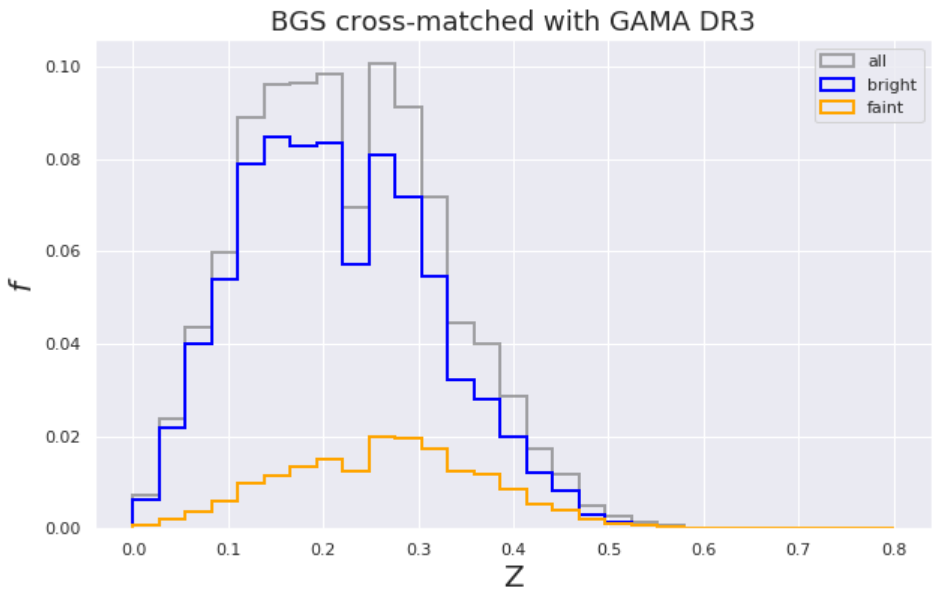
\includegraphics[width=\columnwidth]{images/bgs_gama_z}
    \caption{Redshift distribution of \BGS galaxies cross-matched with \GAMA DR3 broken into bright ($r$-band magnitude lower than $19.5$) and faint ($19.5 < r < 20$) galaxies according to \BGS.  Solid gray shows the overall galaxies.}
    \label{fig:bgs_gama_z}
\end{figure}

DEV models have a sharp profile but wit broader wings than the petrosian model and any other of the \TRACTOR models. The EXP model tend to be less sharp and with less broader wings than the DEV model, however, it still catches more average flux than the petrosian model. REX model is similar to the EXP model but with less flux income. The median values of these models shown negative values, which are relatively small for REX and EXP galaxies, and twice or more bigger for DEV galaxies. This behaviour is expected for $r-\RPETRO$ if the models from the LS \DReight receives more flux income than \GAMA \RPETRO. The story is different for the PSF galaxies that shown a positive offset, meaning that the petrosian model is picking up more flux than the PSF. The positive offset can be understood as errors in the magnitudes due bad fitting of extended sources. We know \TRACTOR force some of their targets to be fitted as PSF only and this might be a consequence of that. Despite the positive values in $r-\RPETRO$ for PSF galaxies, the overall median value is negative ($-0.124$) which means \GAMA \RPETRO magnitude goes $\sim 0.1$ fainter than the $r$ magnitude from the \LS \DReight. 

In terms of redshift, Figure~\ref{fig:bgs_gama_z} shows \GAMA redshift for the cross-matched \BGS and \GAMA objects (solid gray) which represent a target density of $\sim 965$ deg$^{-2}$. We broke the sample into bright (solid blue) and faint (solid orange) \BGS galaxies.


%\subsection{Number counts}
\subsection{Validation of the Star-Galaxy separation in GAMA fields}
\subsubsection{The PSF-type galaxies}

From the the star-galaxy separation definition in section~\ref{subsec:star_galaxy}, we allow some of this galaxies to be PSF best-fit objects by \TRACTOR. We are talking of the order of $4$ deg$^{-2}$ within the \DECaLS footprint. This galaxies present a star behaviour in Figure~\ref{fig:fmc} which makes us question of their galaxy nature. To unveil this, we use \GAMA redshifts. 

\begin{table}
\centering
\begin{tabular}{ |p{2cm}||p{2.5cm}|p{2.5cm}| }
 \hline
 {\bf Sample} & $\eta_{BM}$ [deg$^{-2}$] & $\eta_{AM}$ [deg$^{-2}$] \\
 \hline
 PSF $\&$ BGS & $3.91$ & $1.77$ \\
 \hline
 \hline
 {\bf Subsample} & $f_{BM}$ [$\%$] & $f_{AM}$ [$\%$] \\
 \hline
 $\&$ Not in GAIA  & $39.33$ ($1.54$ deg$^{-2}$) & $1.29$ ($0.02$ deg$^{-2}$) \\
 $\&$ AEN star  & $57.75$ ($2.26$ deg$^{-2}$) & $97.42$ ($1.73$ deg$^{-2}$) \\
 $\&$ AEN galaxy  & $2.92$ ($0.11$ deg$^{-2}$) & $1.29$ ($0.02$ deg$^{-2}$) \\
 \hline
\end{tabular}
\caption{The table shows on top the target density of the PSF-type BGS galaxies within three out of four of the \GAMA fields footprint (G09, G12, G15) before (second column) and after (third column) the cross-match with \GAMA. Subsequent rows show the fraction and target density for disjoint subsamples of the PSF-type BGS sample: not in \GAIA, AEN stars and AEN galaxies.}
\label{tab:bgs_psf_gama}
\end{table}

\begin{figure}
	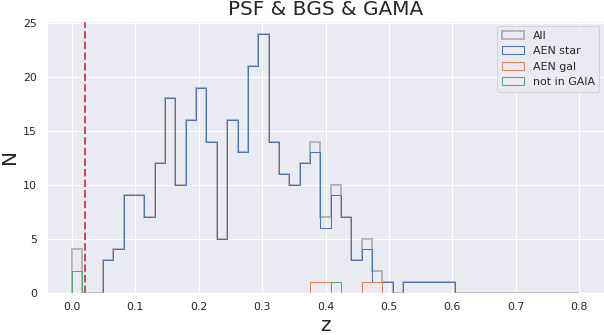
\includegraphics[width=\columnwidth]{images/psf_bgs_gama_redshift}
    \caption{Redshift distribution from \GAMA DR3 of PSF-type BGS galaxies cross-matched with three out of four of the \GAMA fields (G09, G12, G15). The four distributions correspond to the matched sample (gray) and the disjoint subsamples comprising galaxies not in \GAIA (green) and stars and galaxies defined by the AEN classification (blue and red respectively). The red-dashed line points to the redshift star-galaxy separation at $z=0.02$.}
    \label{fig:matched_sample_z}
\end{figure}

First we reduce or \DECaLS footprint of that of \GAMA resulting in a reduced area of $175$ deg$^2$ after accounting for the geometric maskings (i.e., masking around large galaxies, bright stars, globular clusters and completeness in the three bands). The \GAMA fields used are the same G09, G12, G15. Within this footprint, the \BGS PSF-type galaxies (main sample) have a density of $3.91$ deg$^{-2}$ and a density of $1.77$ deg$^{-2}$ after the cross-match (matched sample) with \GAMA. We subdivide the two samples into three disjoint subsamples: not in \GAIA, AEN star and AEN galaxy. The AEN star and AEN galaxy are stars and galaxies defined by the Astrometric Excess Noise classification addressed in appendix~\ref{app:sgmodels}. Results of this are shown in Table~\ref{tab:bgs_psf_gama} where besides the target density of the samples ($\eta_{BM}$ and $\eta_{AM}$), we include the fraction of the subsamples ($f_{BM}$ and $f_{AM}$). The subindex $BM$ and $AM$ refers to before matching and after matching with \GAMA respectively. Our matched sample represent $45 \%$ of the matched sample however, it does not seem to be representative of the main sample with $97 \%$ of its targets classified as AEN stars. Such results suggest a bias is being applied to AEN stars which totally make sense as \TRACTOR force a PSF best-fit to all AEN stars. This would explain the $\sim 58 \%$ of BGS galaxies that has a PSF best-fit but still we have a remain $\sim 42 \%$ which need further investigation. The assumption of \TRACTOR wrongly classifying the stars and galaxies within GAIA using its AEN classification (see Appendix~\ref{app:sgmodels}), and hence wrongly assigning fluxes to such targets, can be corroborate with the \GAMA redshifts. Figure~\ref{fig:matched_sample_z} shows the \GAMA redshifts for the disjoint subsamples of the matched sample. We define the redshift star-galaxy separation at $z=0.02$ \citep{add cite...} and it is clear how almost all the AEN stars well define the \BGS redshift distribution. 

\subsubsection{Assess of \BGS cuts with \GAMA}

\begin{figure}
	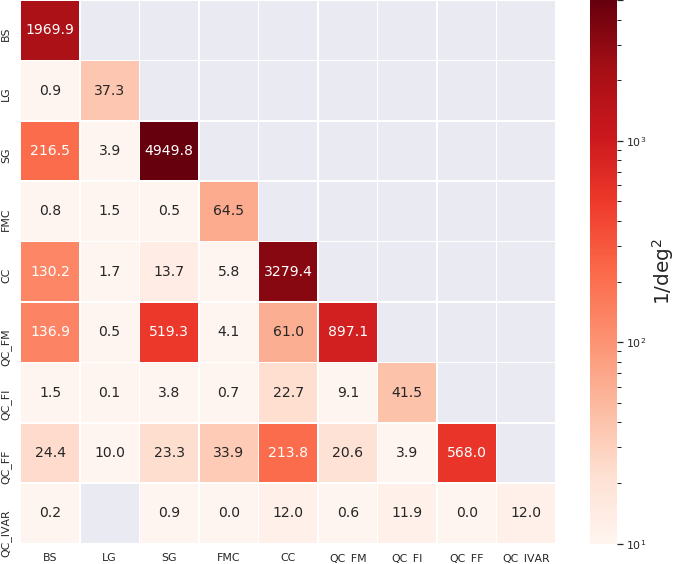
\includegraphics[width=\columnwidth]{images/bgs_rejs_heatmap}
	
	\vspace{1cm}
	
	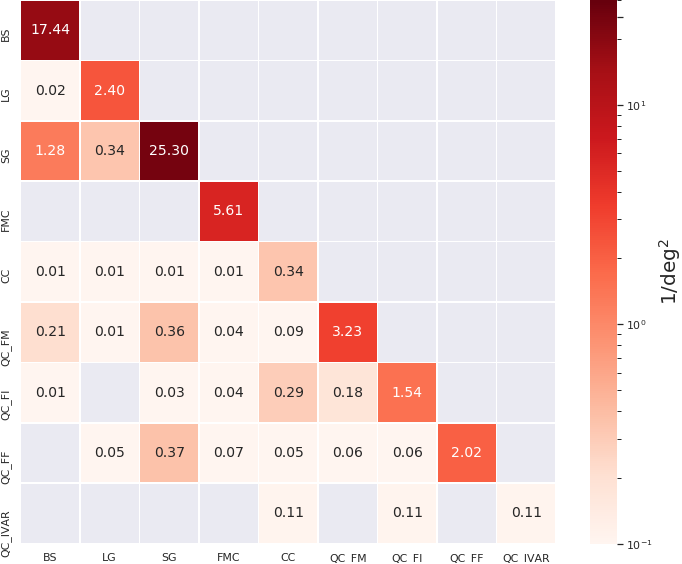
\includegraphics[width=\columnwidth]{images/bgs_rejs_gama_heatmap}
    \caption{Top: Heatmap showing the target density of missed \BGS objects in the reduced LS \DReight. The diagonal quantities are densities by each of the spatial and photometric \BGS cuts while the off-diagonal shows densities of two combined cuts. Bottom: Heatmap showing the subsample of those missed objects that has a cross-match with \GAMA DR3.}
    \label{fig:heatmaps}
\end{figure}

When cross-matching the reduce \DReight with \GAMA DR3, we get a matched target density of $1030.3$ deg$^{-2}$ which represent a fraction of $1.27 \%$ of the reduced \DReight target density and a fraction of $99.6 \%$ of the \GAMA DR3 target density. $948.5$ deg$^{-2}$ out of the $1030.3$ deg$^{-2}$ are \BGS targets and the remain $81.8$ deg$^{-2}$ are missed objects in \BGS due the spatial and photometric cuts we apply, and since the reduced \DReight allows fainter than $r$-mag of $20$, these faint objects are also included in the missed objects density. Figure~\ref{fig:heatmaps} shows heatmaps with the target density rejected by each of the spatial and photometric cuts on the diagonal, and the off-diagonal quantities shows density of missed objects by combinations of two cuts. Top heatmap include missed \BGS objects in the reduced \DReight while bottom heatmap show the subsample of these missed objects that has a cross-match with \GAMA. Besides the huge different in the target density between the missed \BGS in the reduced sample and the same sample corss-matched with \GAMA, the bottom plot, with the \GAMA cross-match, is not a representative sample of missed \BGS from the reduced sample with the exception of the star-galaxy separation rejections that has the highest number in both samples, and objects rejected by the geometric bright star mask. This difference is mainly due the nature of the catalogues where the LS \DReight is way deeper than \GAMA.

\begin{figure}
	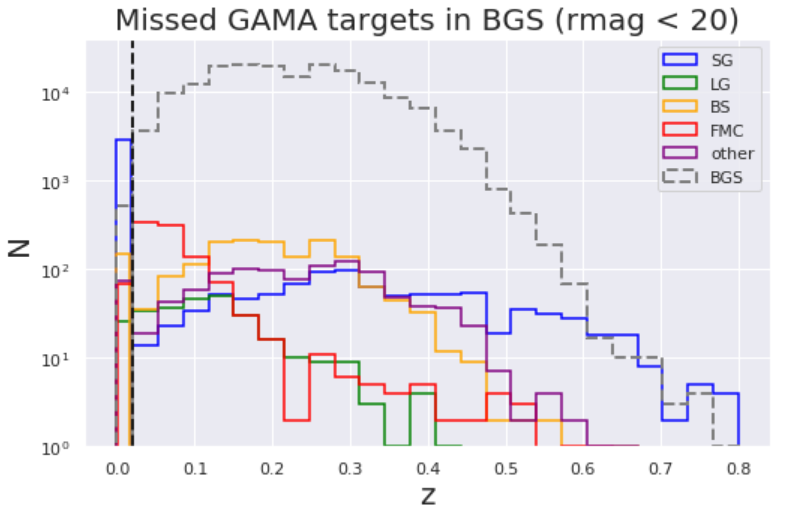
\includegraphics[width=\columnwidth]{images/rejs_gama_redshift}
    \caption{Redshift distribution of missed \GAMA targets in \BGS with LS \DReight $r$-band magnitude below $20$ and broken into the different \BGS rejections categories. Blue solid line shows \GAMA objects missed due star-galaxy separation (SG), green solid due the large galaxy masking (\LG), yellow solid due bright star masking (\BS), red solid due fibre magnitude cut (\FMC) and purple solid due the remain cuts (\CC and \QCs). The dashed gray line shows the redshift distribution of \BGS galaxies cross-matched with \GAMA. Black dashed line divide our sample between \GAMA stars and galaxies at $z=0.02$.}
    \label{fig:rejs_gama_z}
\end{figure}

From bottom heatmap we can see that most of the missed \BGS found in \GAMA are due star-galaxy separation and masking around bright stars. The fact that most of the missed objects are due star-galaxy does not mean that our star-galaxy definition is doing it wrong. In Figure~\ref{fig:rejs_gama_z} we have the \GAMA redshifts distribution of the main \BGS rejections that sum a total target density of $81.8$ deg$^{-2}$. The sample labelled as {\it other} in solid purple is the composition of all the photometric cuts except for the \FMC and star-galaxy separation. The gray dashed line shows the distribution of \BGS cross-matched with \GAMA. Only star-galaxy rejects $29$ deg$^{-2}$ of which $64 \%$ are stars indeed according to \GAMA redshifts and the remain $36 \%$ are galaxies. Such galaxies are close to our threshold limit of our \GAIA star-galaxy separation. We found that $2/3$ of this rejected galaxies are AEN stars meaning that its photometry has been compromised, if they are extended objects as \GAMA points, then their \TRACTOR flux is a fraction of what it really is and hence their magnitude is shifted to fainter values. This translates to lower values in $Grr$ of figure~\ref{fig:Grr-gz} and moving them away of the galaxy locus.

Objects missed by the bright stars masking follows the \BGS shape as well as missed objects by the large galaxies masking which peaks at higher redshifts. \GAMA galaxies within the geometric galaxy mask is expected as \GAMA does not perform a large galaxy masking. However, \GAMA does perform a bright star masking which is less aggressive than the LS \DReight masking, \GAMA bright star masking removes $\sim 1$ deg$^2$ \citep{10.1111/j.1365-2966.2010.16282.x} while LS \DReight removes $\sim 5$ deg$^2$.

Next we have missed galaxies due the \FMC. This include high redshift galaxies and although it also contains some \GAMA stars these are a small fraction (less than $7 \%$). The remain missed \GAMA objects is due colour-colour outliers (\CC) and the quality cuts (\QCs) which represent a total of $\sim 5.8$ deg$^{-2}$ for $r$-band magnitudes below $20$.


%\subsection{Redshift distribution from GAMA}
\subsection{Potential Systematics}
\subsubsection{Mitigation of systematics with linear weights on stellar density}
\subsection{Galaxy clustering with Angular correlation function}
\subsection{Angular cross-correlation with stars}



\iffalse
\subsection{Validating \BGS selection in \GAMA fields}
mag-mag plots. N(z) for the matches. Validate the Star-galaxy separation.


\subsection{\BGS Vs \SDSS classification}
\begin{itemize}
    \item Magnitude comparisons with \SDSS
    \item Number Counts (Alex mock, \SDSS Wang 2013, \BGS test region, \BGS Decals)
    \item Angular Correlation Function ($\omega(\theta$) comparisons with \SDSS and Alex Mock
\end{itemize}

\subsection{Validating the Spatial masking through the Cross-correlations}
\begin{itemize}
    \item Cross-correlations
\end{itemize}

\mike{Survey validation selection?}
\fi

\section{Conclusions}

\section*{Acknowledgements}

The Acknowledgements section is not numbered. Here you can thank helpful
colleagues, acknowledge funding agencies, telescopes and facilities used etc.
Try to keep it short.

%%%%%%%%%%%%%%%%%%%%%%%%%%%%%%%%%%%%%%%%%%%%%%%%%%

%%%%%%%%%%%%%%%%%%%% REFERENCES %%%%%%%%%%%%%%%%%%

% The best way to enter references is to use BibTeX:

\bibliographystyle{mnras}
\bibliography{sample} % if your bibtex file is called example.bib


%%%%%%%%%%%%%%%%%%%%%%%%%%%%%%%%%%%%%%%%%%%%%%%%%%

%%%%%%%%%%%%%%%%% APPENDICES %%%%%%%%%%%%%%%%%%%%%

\appendix
\section{Galaxy view}\label{app:galview}

We present a galaxy view of the \BGS selection criteria by implementing the star-galaxy separation on top of all the \BGS cuts. Results of this are shown in Fig.~\ref{fig:flow_galaxy}. In this view, the geometric masking does not look as aggressive as in Fig.~\ref{fig:flow1} reducing the amount of rejections by a factor of $\sim 6$ being the \BS bit the most affected meaning we have a high number of stars around the bright stars. Then we have \NOBS which seems unaffected by the star-galaxy separation cut. Note that the are removed by these cuts remains unchanged as this does not depend on the number of objects but the randoms.  

In addition to the star-galaxy separation order change compared to the selection criteria presented at sections ~\ref{sec:spatial_masking} and ~\ref{sec:photo_select}, we swap the \FMC with the \QCs. When comparing both orders (Fig.~\ref{fig:flow2} and Fig.~\ref{fig:flow_galaxy}) we see a high overlap between the \QCs and the \FMC of the order of $\sim 18$ deg$^{-2}$ which represent half the galaxies rejected by \FMC in section~\ref{sec:photo_select}. The most overlapped galaxies are between \FRACFLUX and \FMC rejections. 

\omar{elaborate on why such overlap between \FRACFLUX and \FMC ?}

\begin{figure*}
	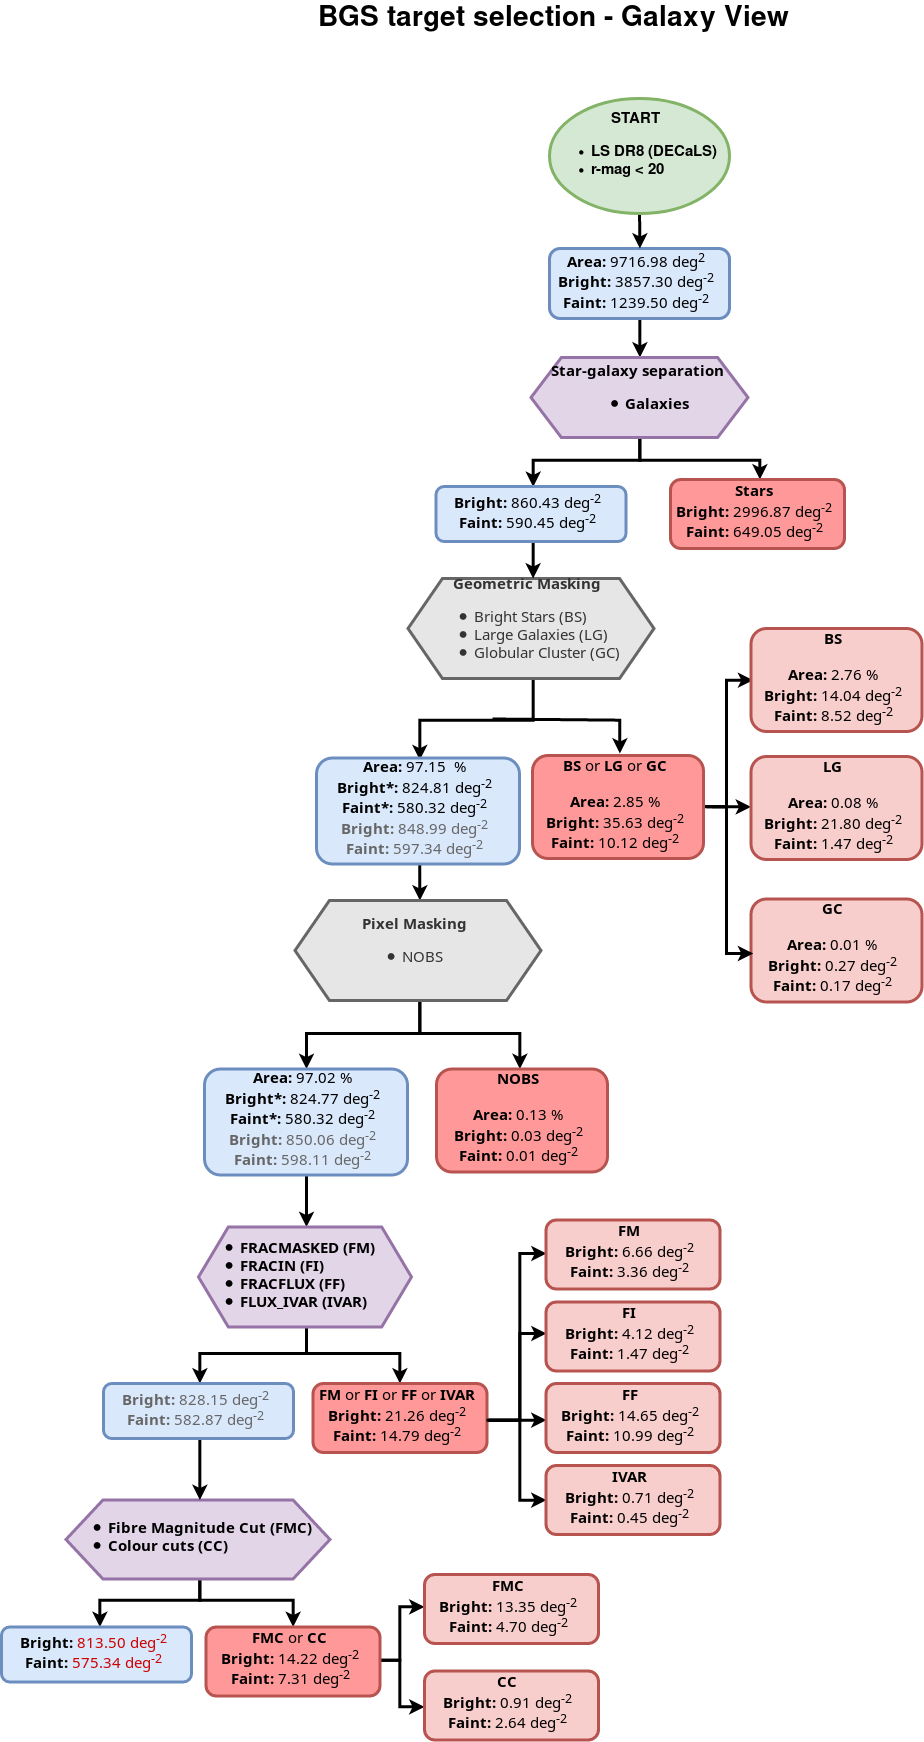
\includegraphics[width=10.7cm]{images/flow_galaxy.png}
    \caption{Flow chart that shows the Spatial and Photometric \BGS target selections in \DECaLS data from the Legacy Survey \DReight. The spatial selection of \BGS targets are shown in gray and are divided in two kinds, one defined by the geometric-based cuts around the bright sources i.e., Bright Stars (\BS), Large Galaxies (\LG) and Globular Clusters (\GC), and by pixel-based cuts such as the number of observations (\NOBS). The photometric selection of \BGS targets is divided in four kinds; Star-Galaxy separation, Fibre Magnitude Cuts (\FMC), Colour Cuts (\CC) and Quality Cuts (\QCs) defined by \FRACMASKED, \FRACIN, \FRACFLUX and \FLUXIVAR. The blue boxes show the resulted kept objects in terms of the area (in degrees) and number density (per square degree) broken into bright and faint before and after each of the \BGS cuts classes, while the red boxes shown the same information but for the rejected objects. If more than one type of masking is presented at each stage (each of the gray or purple hexagons), then the dark-red boxes show the results for the combination of the masks avoiding overlaps (as it is the case of the Geometric Masking and the last two photometric cuts) and the light-red boxes shows the results for each individual mask. The upper ($^*$) in blue rectangles shows the target densities without the corrected area by previous masks while densities with not upper ($^*$) does account for previous masking for the area.}
    \label{fig:flow_galaxy}
\end{figure*}


\section{Comparison of Star-Galaxy separation with AEN and Grr}\label{app:sgmodels}

For objects detected in \GAIA, \TRACTOR and \BGS have adopted different star-galaxy classification methods. \BGS uses the difference in the \GAIA $G$-band magnitude and the \TRACTOR raw $r$-band magnitude (not corrected for extinction) as a measure of how extended the object is (see section~\ref{subsec:star_galaxy}). In contrast, Tractor makes use of the \GAIA Astrometric Excess noise (AEN) parameter. The agreement between these two definitions is not perfect and this is an issue as some objects that \BGS classifies as galaxies ($\sim 6$ deg$^{-2}$) \TRACTOR treats as stars and only measures PSF magnitudes.

Tractor only fits PSF models to \GAIA objects it classifies as stars. Namely those that satisfy the following conditions:

\begin{equation}
	\begin{cases}
      AEN < 10^{0.5}, & G \leq 19\\
      AEN < 10^{0.5 + 0.2(G - 19)}, & G \geq 19.\\
	\end{cases}
\end{equation}

$G$ is the \GAIA photometric $G$-band. We refer to this classification as AEN classification. 



\iffalse
\section{Some extra material}

in context, cites relevant earlier studies in the field by \citet{Others2013},
and describes the problem the authors aim to solve \citep[e.g.][]{Author2012}.

\begin{equation}
    x=\frac{-b\pm\sqrt{b^2-4ac}}{2a}.
	\label{eq:quadratic}
\end{equation}

Refer back to them as e.g. equation~(\ref{eq:quadratic}).

Figures are referred to as e.g. Fig.~\ref{fig:example_figure}, and tables as
e.g. Table~\ref{tab:example_table}.

% Example figure
\begin{figure}
	% To include a figure from a file named example.*
	% Allowable file formats are eps or ps if compiling using latex
	% or pdf, png, jpg if compiling using pdflatex
	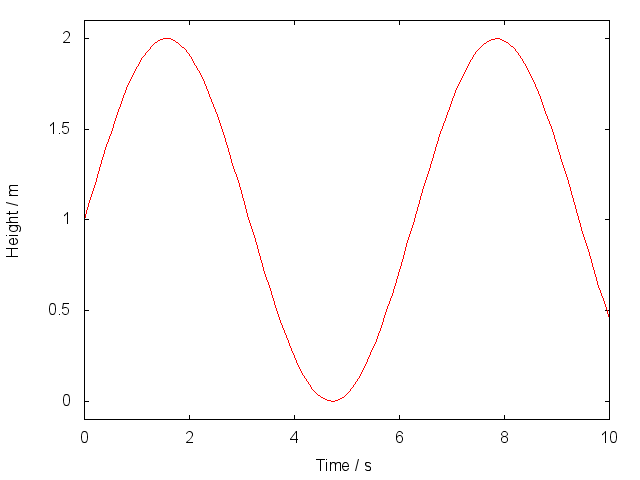
\includegraphics[width=\columnwidth]{example}
    \caption{This is an example figure. Captions appear below each figure.
	Give enough detail for the reader to understand what they're looking at,
	but leave detailed discussion to the main body of the text.}
    \label{fig:example_figure}
\end{figure}

% Example table
\begin{table}
	\centering
	\caption{This is an example table. Captions appear above each table.
	Remember to define the quantities, symbols and units used.}
	\label{tab:example_table}
	\begin{tabular}{lccr} % four columns, alignment for each
		\hline
		A & B & C & D\\
		\hline
		1 & 2 & 3 & 4\\
		2 & 4 & 6 & 8\\
		3 & 5 & 7 & 9\\
		\hline
	\end{tabular}
\end{table}

\fi
%%%%%%%%%%%%%%%%%%%%%%%%%%%%%%%%%%%%%%%%%%%%%%%%%%


% Don't change these lines
\bsp	% typesetting comment
\label{lastpage}
\end{document}

% End of mnras_template.tex\\ 




